\documentclass[11pt]{article}

%\usepackage[T2A]{fontenc}
%\usepackage[utf8]{inputenc}
%\usepackage[english, russian]{babel}

\usepackage[breakable]{tcolorbox}
    \usepackage{parskip} % Stop auto-indenting (to mimic markdown behaviour)
    
    \usepackage{iftex}
    \ifPDFTeX
    	\usepackage[T1]{fontenc}
    	\usepackage{mathpazo}
    \else
    	\usepackage{fontspec}
    \fi

    % Basic figure setup, for now with no caption control since it's done
    % automatically by Pandoc (which extracts ![](path) syntax from Markdown).
    \usepackage{graphicx}
    % Maintain compatibility with old templates. Remove in nbconvert 6.0
    \let\Oldincludegraphics\includegraphics
    % Ensure that by default, figures have no caption (until we provide a
    % proper Figure object with a Caption API and a way to capture that
    % in the conversion process - todo).
    \usepackage{caption}
    \DeclareCaptionFormat{nocaption}{}
    \captionsetup{format=nocaption,aboveskip=0pt,belowskip=0pt}

    \usepackage{float}
    \floatplacement{figure}{H} % forces figures to be placed at the correct location
    \usepackage{xcolor} % Allow colors to be defined
    \usepackage{enumerate} % Needed for markdown enumerations to work
    \usepackage{geometry} % Used to adjust the document margins
    \usepackage{amsmath} % Equations
    \usepackage{amssymb} % Equations
    \usepackage{textcomp} % defines textquotesingle
    % Hack from http://tex.stackexchange.com/a/47451/13684:
    \AtBeginDocument{%
        \def\PYZsq{\textquotesingle}% Upright quotes in Pygmentized code
    }
    \usepackage{upquote} % Upright quotes for verbatim code
    \usepackage{eurosym} % defines \euro
    \usepackage[mathletters]{ucs} % Extended unicode (utf-8) support
    \usepackage{fancyvrb} % verbatim replacement that allows latex
    \usepackage{grffile} % extends the file name processing of package graphics 
                         % to support a larger range
    \makeatletter % fix for old versions of grffile with XeLaTeX
    \@ifpackagelater{grffile}{2019/11/01}
    {
      % Do nothing on new versions
    }
    {
      \def\Gread@@xetex#1{%
        \IfFileExists{"\Gin@base".bb}%
        {\Gread@eps{\Gin@base.bb}}%
        {\Gread@@xetex@aux#1}%
      }
    }
    \makeatother
    \usepackage[Export]{adjustbox} % Used to constrain images to a maximum size
    \adjustboxset{max size={0.9\linewidth}{0.9\paperheight}}

    % The hyperref package gives us a pdf with properly built
    % internal navigation ('pdf bookmarks' for the table of contents,
    % internal cross-reference links, web links for URLs, etc.)
    \usepackage{hyperref}
    % The default LaTeX title has an obnoxious amount of whitespace. By default,
    % titling removes some of it. It also provides customization options.
    \usepackage{titling}
    \usepackage{longtable} % longtable support required by pandoc >1.10
    \usepackage{booktabs}  % table support for pandoc > 1.12.2
    \usepackage[inline]{enumitem} % IRkernel/repr support (it uses the enumerate* environment)
    \usepackage[normalem]{ulem} % ulem is needed to support strikethroughs (\sout)
                                % normalem makes italics be italics, not underlines
    \usepackage{mathrsfs}
    
\usepackage{wrapfig}
\usepackage[rightcaption]{sidecap}
\providecommand{\keywords}[1]{\textbf{\textit{Keywords:}} #1}

\author{A. Ju. Drozdov}

    
    % Colors for the hyperref package
    \definecolor{urlcolor}{rgb}{0,.145,.698}
    \definecolor{linkcolor}{rgb}{.71,0.21,0.01}
    \definecolor{citecolor}{rgb}{.12,.54,.11}

    % ANSI colors
    \definecolor{ansi-black}{HTML}{3E424D}
    \definecolor{ansi-black-intense}{HTML}{282C36}
    \definecolor{ansi-red}{HTML}{E75C58}
    \definecolor{ansi-red-intense}{HTML}{B22B31}
    \definecolor{ansi-green}{HTML}{00A250}
    \definecolor{ansi-green-intense}{HTML}{007427}
    \definecolor{ansi-yellow}{HTML}{DDB62B}
    \definecolor{ansi-yellow-intense}{HTML}{B27D12}
    \definecolor{ansi-blue}{HTML}{208FFB}
    \definecolor{ansi-blue-intense}{HTML}{0065CA}
    \definecolor{ansi-magenta}{HTML}{D160C4}
    \definecolor{ansi-magenta-intense}{HTML}{A03196}
    \definecolor{ansi-cyan}{HTML}{60C6C8}
    \definecolor{ansi-cyan-intense}{HTML}{258F8F}
    \definecolor{ansi-white}{HTML}{C5C1B4}
    \definecolor{ansi-white-intense}{HTML}{A1A6B2}
    \definecolor{ansi-default-inverse-fg}{HTML}{FFFFFF}
    \definecolor{ansi-default-inverse-bg}{HTML}{000000}

    % common color for the border for error outputs.
    \definecolor{outerrorbackground}{HTML}{FFDFDF}

    % commands and environments needed by pandoc snippets
    % extracted from the output of `pandoc -s`
    \providecommand{\tightlist}{%
      \setlength{\itemsep}{0pt}\setlength{\parskip}{0pt}}
    \DefineVerbatimEnvironment{Highlighting}{Verbatim}{commandchars=\\\{\}}
    % Add ',fontsize=\small' for more characters per line
    \newenvironment{Shaded}{}{}
    \newcommand{\KeywordTok}[1]{\textcolor[rgb]{0.00,0.44,0.13}{\textbf{{#1}}}}
    \newcommand{\DataTypeTok}[1]{\textcolor[rgb]{0.56,0.13,0.00}{{#1}}}
    \newcommand{\DecValTok}[1]{\textcolor[rgb]{0.25,0.63,0.44}{{#1}}}
    \newcommand{\BaseNTok}[1]{\textcolor[rgb]{0.25,0.63,0.44}{{#1}}}
    \newcommand{\FloatTok}[1]{\textcolor[rgb]{0.25,0.63,0.44}{{#1}}}
    \newcommand{\CharTok}[1]{\textcolor[rgb]{0.25,0.44,0.63}{{#1}}}
    \newcommand{\StringTok}[1]{\textcolor[rgb]{0.25,0.44,0.63}{{#1}}}
    \newcommand{\CommentTok}[1]{\textcolor[rgb]{0.38,0.63,0.69}{\textit{{#1}}}}
    \newcommand{\OtherTok}[1]{\textcolor[rgb]{0.00,0.44,0.13}{{#1}}}
    \newcommand{\AlertTok}[1]{\textcolor[rgb]{1.00,0.00,0.00}{\textbf{{#1}}}}
    \newcommand{\FunctionTok}[1]{\textcolor[rgb]{0.02,0.16,0.49}{{#1}}}
    \newcommand{\RegionMarkerTok}[1]{{#1}}
    \newcommand{\ErrorTok}[1]{\textcolor[rgb]{1.00,0.00,0.00}{\textbf{{#1}}}}
    \newcommand{\NormalTok}[1]{{#1}}
    
    % Additional commands for more recent versions of Pandoc
    \newcommand{\ConstantTok}[1]{\textcolor[rgb]{0.53,0.00,0.00}{{#1}}}
    \newcommand{\SpecialCharTok}[1]{\textcolor[rgb]{0.25,0.44,0.63}{{#1}}}
    \newcommand{\VerbatimStringTok}[1]{\textcolor[rgb]{0.25,0.44,0.63}{{#1}}}
    \newcommand{\SpecialStringTok}[1]{\textcolor[rgb]{0.73,0.40,0.53}{{#1}}}
    \newcommand{\ImportTok}[1]{{#1}}
    \newcommand{\DocumentationTok}[1]{\textcolor[rgb]{0.73,0.13,0.13}{\textit{{#1}}}}
    \newcommand{\AnnotationTok}[1]{\textcolor[rgb]{0.38,0.63,0.69}{\textbf{\textit{{#1}}}}}
    \newcommand{\CommentVarTok}[1]{\textcolor[rgb]{0.38,0.63,0.69}{\textbf{\textit{{#1}}}}}
    \newcommand{\VariableTok}[1]{\textcolor[rgb]{0.10,0.09,0.49}{{#1}}}
    \newcommand{\ControlFlowTok}[1]{\textcolor[rgb]{0.00,0.44,0.13}{\textbf{{#1}}}}
    \newcommand{\OperatorTok}[1]{\textcolor[rgb]{0.40,0.40,0.40}{{#1}}}
    \newcommand{\BuiltInTok}[1]{{#1}}
    \newcommand{\ExtensionTok}[1]{{#1}}
    \newcommand{\PreprocessorTok}[1]{\textcolor[rgb]{0.74,0.48,0.00}{{#1}}}
    \newcommand{\AttributeTok}[1]{\textcolor[rgb]{0.49,0.56,0.16}{{#1}}}
    \newcommand{\InformationTok}[1]{\textcolor[rgb]{0.38,0.63,0.69}{\textbf{\textit{{#1}}}}}
    \newcommand{\WarningTok}[1]{\textcolor[rgb]{0.38,0.63,0.69}{\textbf{\textit{{#1}}}}}
    
    
    % Define a nice break command that doesn't care if a line doesn't already
    % exist.
    \def\br{\hspace*{\fill} \\* }
    % Math Jax compatibility definitions
    \def\gt{>}
    \def\lt{<}
    \let\Oldtex\TeX
    \let\Oldlatex\LaTeX
    \renewcommand{\TeX}{\textrm{\Oldtex}}
    \renewcommand{\LaTeX}{\textrm{\Oldlatex}}
    % Document parameters
    % Document title
    \title{Casimir honeycomb drive: On the force on different sides of perfectly conducting honeycomb on a plate.}
    
    
    
% Pygments definitions
\makeatletter
\def\PY@reset{\let\PY@it=\relax \let\PY@bf=\relax%
    \let\PY@ul=\relax \let\PY@tc=\relax%
    \let\PY@bc=\relax \let\PY@ff=\relax}
\def\PY@tok#1{\csname PY@tok@#1\endcsname}
\def\PY@toks#1+{\ifx\relax#1\empty\else%
    \PY@tok{#1}\expandafter\PY@toks\fi}
\def\PY@do#1{\PY@bc{\PY@tc{\PY@ul{%
    \PY@it{\PY@bf{\PY@ff{#1}}}}}}}
\def\PY#1#2{\PY@reset\PY@toks#1+\relax+\PY@do{#2}}

\@namedef{PY@tok@w}{\def\PY@tc##1{\textcolor[rgb]{0.73,0.73,0.73}{##1}}}
\@namedef{PY@tok@c}{\let\PY@it=\textit\def\PY@tc##1{\textcolor[rgb]{0.25,0.50,0.50}{##1}}}
\@namedef{PY@tok@cp}{\def\PY@tc##1{\textcolor[rgb]{0.74,0.48,0.00}{##1}}}
\@namedef{PY@tok@k}{\let\PY@bf=\textbf\def\PY@tc##1{\textcolor[rgb]{0.00,0.50,0.00}{##1}}}
\@namedef{PY@tok@kp}{\def\PY@tc##1{\textcolor[rgb]{0.00,0.50,0.00}{##1}}}
\@namedef{PY@tok@kt}{\def\PY@tc##1{\textcolor[rgb]{0.69,0.00,0.25}{##1}}}
\@namedef{PY@tok@o}{\def\PY@tc##1{\textcolor[rgb]{0.40,0.40,0.40}{##1}}}
\@namedef{PY@tok@ow}{\let\PY@bf=\textbf\def\PY@tc##1{\textcolor[rgb]{0.67,0.13,1.00}{##1}}}
\@namedef{PY@tok@nb}{\def\PY@tc##1{\textcolor[rgb]{0.00,0.50,0.00}{##1}}}
\@namedef{PY@tok@nf}{\def\PY@tc##1{\textcolor[rgb]{0.00,0.00,1.00}{##1}}}
\@namedef{PY@tok@nc}{\let\PY@bf=\textbf\def\PY@tc##1{\textcolor[rgb]{0.00,0.00,1.00}{##1}}}
\@namedef{PY@tok@nn}{\let\PY@bf=\textbf\def\PY@tc##1{\textcolor[rgb]{0.00,0.00,1.00}{##1}}}
\@namedef{PY@tok@ne}{\let\PY@bf=\textbf\def\PY@tc##1{\textcolor[rgb]{0.82,0.25,0.23}{##1}}}
\@namedef{PY@tok@nv}{\def\PY@tc##1{\textcolor[rgb]{0.10,0.09,0.49}{##1}}}
\@namedef{PY@tok@no}{\def\PY@tc##1{\textcolor[rgb]{0.53,0.00,0.00}{##1}}}
\@namedef{PY@tok@nl}{\def\PY@tc##1{\textcolor[rgb]{0.63,0.63,0.00}{##1}}}
\@namedef{PY@tok@ni}{\let\PY@bf=\textbf\def\PY@tc##1{\textcolor[rgb]{0.60,0.60,0.60}{##1}}}
\@namedef{PY@tok@na}{\def\PY@tc##1{\textcolor[rgb]{0.49,0.56,0.16}{##1}}}
\@namedef{PY@tok@nt}{\let\PY@bf=\textbf\def\PY@tc##1{\textcolor[rgb]{0.00,0.50,0.00}{##1}}}
\@namedef{PY@tok@nd}{\def\PY@tc##1{\textcolor[rgb]{0.67,0.13,1.00}{##1}}}
\@namedef{PY@tok@s}{\def\PY@tc##1{\textcolor[rgb]{0.73,0.13,0.13}{##1}}}
\@namedef{PY@tok@sd}{\let\PY@it=\textit\def\PY@tc##1{\textcolor[rgb]{0.73,0.13,0.13}{##1}}}
\@namedef{PY@tok@si}{\let\PY@bf=\textbf\def\PY@tc##1{\textcolor[rgb]{0.73,0.40,0.53}{##1}}}
\@namedef{PY@tok@se}{\let\PY@bf=\textbf\def\PY@tc##1{\textcolor[rgb]{0.73,0.40,0.13}{##1}}}
\@namedef{PY@tok@sr}{\def\PY@tc##1{\textcolor[rgb]{0.73,0.40,0.53}{##1}}}
\@namedef{PY@tok@ss}{\def\PY@tc##1{\textcolor[rgb]{0.10,0.09,0.49}{##1}}}
\@namedef{PY@tok@sx}{\def\PY@tc##1{\textcolor[rgb]{0.00,0.50,0.00}{##1}}}
\@namedef{PY@tok@m}{\def\PY@tc##1{\textcolor[rgb]{0.40,0.40,0.40}{##1}}}
\@namedef{PY@tok@gh}{\let\PY@bf=\textbf\def\PY@tc##1{\textcolor[rgb]{0.00,0.00,0.50}{##1}}}
\@namedef{PY@tok@gu}{\let\PY@bf=\textbf\def\PY@tc##1{\textcolor[rgb]{0.50,0.00,0.50}{##1}}}
\@namedef{PY@tok@gd}{\def\PY@tc##1{\textcolor[rgb]{0.63,0.00,0.00}{##1}}}
\@namedef{PY@tok@gi}{\def\PY@tc##1{\textcolor[rgb]{0.00,0.63,0.00}{##1}}}
\@namedef{PY@tok@gr}{\def\PY@tc##1{\textcolor[rgb]{1.00,0.00,0.00}{##1}}}
\@namedef{PY@tok@ge}{\let\PY@it=\textit}
\@namedef{PY@tok@gs}{\let\PY@bf=\textbf}
\@namedef{PY@tok@gp}{\let\PY@bf=\textbf\def\PY@tc##1{\textcolor[rgb]{0.00,0.00,0.50}{##1}}}
\@namedef{PY@tok@go}{\def\PY@tc##1{\textcolor[rgb]{0.53,0.53,0.53}{##1}}}
\@namedef{PY@tok@gt}{\def\PY@tc##1{\textcolor[rgb]{0.00,0.27,0.87}{##1}}}
\@namedef{PY@tok@err}{\def\PY@bc##1{{\setlength{\fboxsep}{\string -\fboxrule}\fcolorbox[rgb]{1.00,0.00,0.00}{1,1,1}{\strut ##1}}}}
\@namedef{PY@tok@kc}{\let\PY@bf=\textbf\def\PY@tc##1{\textcolor[rgb]{0.00,0.50,0.00}{##1}}}
\@namedef{PY@tok@kd}{\let\PY@bf=\textbf\def\PY@tc##1{\textcolor[rgb]{0.00,0.50,0.00}{##1}}}
\@namedef{PY@tok@kn}{\let\PY@bf=\textbf\def\PY@tc##1{\textcolor[rgb]{0.00,0.50,0.00}{##1}}}
\@namedef{PY@tok@kr}{\let\PY@bf=\textbf\def\PY@tc##1{\textcolor[rgb]{0.00,0.50,0.00}{##1}}}
\@namedef{PY@tok@bp}{\def\PY@tc##1{\textcolor[rgb]{0.00,0.50,0.00}{##1}}}
\@namedef{PY@tok@fm}{\def\PY@tc##1{\textcolor[rgb]{0.00,0.00,1.00}{##1}}}
\@namedef{PY@tok@vc}{\def\PY@tc##1{\textcolor[rgb]{0.10,0.09,0.49}{##1}}}
\@namedef{PY@tok@vg}{\def\PY@tc##1{\textcolor[rgb]{0.10,0.09,0.49}{##1}}}
\@namedef{PY@tok@vi}{\def\PY@tc##1{\textcolor[rgb]{0.10,0.09,0.49}{##1}}}
\@namedef{PY@tok@vm}{\def\PY@tc##1{\textcolor[rgb]{0.10,0.09,0.49}{##1}}}
\@namedef{PY@tok@sa}{\def\PY@tc##1{\textcolor[rgb]{0.73,0.13,0.13}{##1}}}
\@namedef{PY@tok@sb}{\def\PY@tc##1{\textcolor[rgb]{0.73,0.13,0.13}{##1}}}
\@namedef{PY@tok@sc}{\def\PY@tc##1{\textcolor[rgb]{0.73,0.13,0.13}{##1}}}
\@namedef{PY@tok@dl}{\def\PY@tc##1{\textcolor[rgb]{0.73,0.13,0.13}{##1}}}
\@namedef{PY@tok@s2}{\def\PY@tc##1{\textcolor[rgb]{0.73,0.13,0.13}{##1}}}
\@namedef{PY@tok@sh}{\def\PY@tc##1{\textcolor[rgb]{0.73,0.13,0.13}{##1}}}
\@namedef{PY@tok@s1}{\def\PY@tc##1{\textcolor[rgb]{0.73,0.13,0.13}{##1}}}
\@namedef{PY@tok@mb}{\def\PY@tc##1{\textcolor[rgb]{0.40,0.40,0.40}{##1}}}
\@namedef{PY@tok@mf}{\def\PY@tc##1{\textcolor[rgb]{0.40,0.40,0.40}{##1}}}
\@namedef{PY@tok@mh}{\def\PY@tc##1{\textcolor[rgb]{0.40,0.40,0.40}{##1}}}
\@namedef{PY@tok@mi}{\def\PY@tc##1{\textcolor[rgb]{0.40,0.40,0.40}{##1}}}
\@namedef{PY@tok@il}{\def\PY@tc##1{\textcolor[rgb]{0.40,0.40,0.40}{##1}}}
\@namedef{PY@tok@mo}{\def\PY@tc##1{\textcolor[rgb]{0.40,0.40,0.40}{##1}}}
\@namedef{PY@tok@ch}{\let\PY@it=\textit\def\PY@tc##1{\textcolor[rgb]{0.25,0.50,0.50}{##1}}}
\@namedef{PY@tok@cm}{\let\PY@it=\textit\def\PY@tc##1{\textcolor[rgb]{0.25,0.50,0.50}{##1}}}
\@namedef{PY@tok@cpf}{\let\PY@it=\textit\def\PY@tc##1{\textcolor[rgb]{0.25,0.50,0.50}{##1}}}
\@namedef{PY@tok@c1}{\let\PY@it=\textit\def\PY@tc##1{\textcolor[rgb]{0.25,0.50,0.50}{##1}}}
\@namedef{PY@tok@cs}{\let\PY@it=\textit\def\PY@tc##1{\textcolor[rgb]{0.25,0.50,0.50}{##1}}}

\def\PYZbs{\char`\\}
\def\PYZus{\char`\_}
\def\PYZob{\char`\{}
\def\PYZcb{\char`\}}
\def\PYZca{\char`\^}
\def\PYZam{\char`\&}
\def\PYZlt{\char`\<}
\def\PYZgt{\char`\>}
\def\PYZsh{\char`\#}
\def\PYZpc{\char`\%}
\def\PYZdl{\char`\$}
\def\PYZhy{\char`\-}
\def\PYZsq{\char`\'}
\def\PYZdq{\char`\"}
\def\PYZti{\char`\~}
% for compatibility with earlier versions
\def\PYZat{@}
\def\PYZlb{[}
\def\PYZrb{]}
\makeatother


    % For linebreaks inside Verbatim environment from package fancyvrb. 
    \makeatletter
        \newbox\Wrappedcontinuationbox 
        \newbox\Wrappedvisiblespacebox 
        \newcommand*\Wrappedvisiblespace {\textcolor{red}{\textvisiblespace}} 
        \newcommand*\Wrappedcontinuationsymbol {\textcolor{red}{\llap{\tiny$\m@th\hookrightarrow$}}} 
        \newcommand*\Wrappedcontinuationindent {3ex } 
        \newcommand*\Wrappedafterbreak {\kern\Wrappedcontinuationindent\copy\Wrappedcontinuationbox} 
        % Take advantage of the already applied Pygments mark-up to insert 
        % potential linebreaks for TeX processing. 
        %        {, <, #, %, $, ' and ": go to next line. 
        %        _, }, ^, &, >, - and ~: stay at end of broken line. 
        % Use of \textquotesingle for straight quote. 
        \newcommand*\Wrappedbreaksatspecials {% 
            \def\PYGZus{\discretionary{\char`\_}{\Wrappedafterbreak}{\char`\_}}% 
            \def\PYGZob{\discretionary{}{\Wrappedafterbreak\char`\{}{\char`\{}}% 
            \def\PYGZcb{\discretionary{\char`\}}{\Wrappedafterbreak}{\char`\}}}% 
            \def\PYGZca{\discretionary{\char`\^}{\Wrappedafterbreak}{\char`\^}}% 
            \def\PYGZam{\discretionary{\char`\&}{\Wrappedafterbreak}{\char`\&}}% 
            \def\PYGZlt{\discretionary{}{\Wrappedafterbreak\char`\<}{\char`\<}}% 
            \def\PYGZgt{\discretionary{\char`\>}{\Wrappedafterbreak}{\char`\>}}% 
            \def\PYGZsh{\discretionary{}{\Wrappedafterbreak\char`\#}{\char`\#}}% 
            \def\PYGZpc{\discretionary{}{\Wrappedafterbreak\char`\%}{\char`\%}}% 
            \def\PYGZdl{\discretionary{}{\Wrappedafterbreak\char`\$}{\char`\$}}% 
            \def\PYGZhy{\discretionary{\char`\-}{\Wrappedafterbreak}{\char`\-}}% 
            \def\PYGZsq{\discretionary{}{\Wrappedafterbreak\textquotesingle}{\textquotesingle}}% 
            \def\PYGZdq{\discretionary{}{\Wrappedafterbreak\char`\"}{\char`\"}}% 
            \def\PYGZti{\discretionary{\char`\~}{\Wrappedafterbreak}{\char`\~}}% 
        } 
        % Some characters . , ; ? ! / are not pygmentized. 
        % This macro makes them "active" and they will insert potential linebreaks 
        \newcommand*\Wrappedbreaksatpunct {% 
            \lccode`\~`\.\lowercase{\def~}{\discretionary{\hbox{\char`\.}}{\Wrappedafterbreak}{\hbox{\char`\.}}}% 
            \lccode`\~`\,\lowercase{\def~}{\discretionary{\hbox{\char`\,}}{\Wrappedafterbreak}{\hbox{\char`\,}}}% 
            \lccode`\~`\;\lowercase{\def~}{\discretionary{\hbox{\char`\;}}{\Wrappedafterbreak}{\hbox{\char`\;}}}% 
            \lccode`\~`\:\lowercase{\def~}{\discretionary{\hbox{\char`\:}}{\Wrappedafterbreak}{\hbox{\char`\:}}}% 
            \lccode`\~`\?\lowercase{\def~}{\discretionary{\hbox{\char`\?}}{\Wrappedafterbreak}{\hbox{\char`\?}}}% 
            \lccode`\~`\!\lowercase{\def~}{\discretionary{\hbox{\char`\!}}{\Wrappedafterbreak}{\hbox{\char`\!}}}% 
            \lccode`\~`\/\lowercase{\def~}{\discretionary{\hbox{\char`\/}}{\Wrappedafterbreak}{\hbox{\char`\/}}}% 
            \catcode`\.\active
            \catcode`\,\active 
            \catcode`\;\active
            \catcode`\:\active
            \catcode`\?\active
            \catcode`\!\active
            \catcode`\/\active 
            \lccode`\~`\~ 	
        }
    \makeatother

    \let\OriginalVerbatim=\Verbatim
    \makeatletter
    \renewcommand{\Verbatim}[1][1]{%
        %\parskip\z@skip
        \sbox\Wrappedcontinuationbox {\Wrappedcontinuationsymbol}%
        \sbox\Wrappedvisiblespacebox {\FV@SetupFont\Wrappedvisiblespace}%
        \def\FancyVerbFormatLine ##1{\hsize\linewidth
            \vtop{\raggedright\hyphenpenalty\z@\exhyphenpenalty\z@
                \doublehyphendemerits\z@\finalhyphendemerits\z@
                \strut ##1\strut}%
        }%
        % If the linebreak is at a space, the latter will be displayed as visible
        % space at end of first line, and a continuation symbol starts next line.
        % Stretch/shrink are however usually zero for typewriter font.
        \def\FV@Space {%
            \nobreak\hskip\z@ plus\fontdimen3\font minus\fontdimen4\font
            \discretionary{\copy\Wrappedvisiblespacebox}{\Wrappedafterbreak}
            {\kern\fontdimen2\font}%
        }%
        
        % Allow breaks at special characters using \PYG... macros.
        \Wrappedbreaksatspecials
        % Breaks at punctuation characters . , ; ? ! and / need catcode=\active 	
        \OriginalVerbatim[#1,codes*=\Wrappedbreaksatpunct]%
    }
    \makeatother

    % Exact colors from NB
    \definecolor{incolor}{HTML}{303F9F}
    \definecolor{outcolor}{HTML}{D84315}
    \definecolor{cellborder}{HTML}{CFCFCF}
    \definecolor{cellbackground}{HTML}{F7F7F7}
    
    % prompt
    \makeatletter
    \newcommand{\boxspacing}{\kern\kvtcb@left@rule\kern\kvtcb@boxsep}
    \makeatother
    \newcommand{\prompt}[4]{
        {\ttfamily\llap{{\color{#2}[#3]:\hspace{3pt}#4}}\vspace{-\baselineskip}}
    }
    

    
    % Prevent overflowing lines due to hard-to-break entities
    \sloppy 
    % Setup hyperref package
    \hypersetup{
      breaklinks=true,  % so long urls are correctly broken across lines
      colorlinks=true,
      urlcolor=urlcolor,
      linkcolor=linkcolor,
      citecolor=citecolor,
      }
    % Slightly bigger margins than the latex defaults
    
    \geometry{verbose,tmargin=1in,bmargin=1in,lmargin=1in,rmargin=1in}
    
    

\begin{document}
    
    \maketitle
    
    

    
    \title{Casimir honeycomb drive: On the force on different sides of perfectly conducting honeycomb on a plate.}

    \begin{abstract}

By analogy with the classical one dimensional two body Casimir effect, when the pushing in Casimir forces acts on each of the two plates as the difference in electromagnetic pressures of zero-point quantum vacuum oscillations on opposite sides of each of the plates, due to the fact that the geometry vacuum resonator in the inner and outer regions is different, one can try to create a difference in electromagnetic pressures of quantum vacuum oscillations on different sides of only one plate due to the difference in the geometry of vacuum resonators on both sides of it. To do this, nanocells must be grown on one of the surfaces of a smooth metal plate.

Two dimensional one body Casimir effect on square-shaped nanocells was analyzed in this work. As result it was found that the formula for force per unit and for energy density difference per square unit $F/S \approx \delta\left(E/V\right) = R\left(a k_m\right)\cdot\left(\hbar\,c\,\pi/{a^4}\right)$ is very similar to the formula of the classical Casimir effect except for the proportionality factor's value.

\end{abstract}

    \begin{keywords}
Two dimensional one body Casimir effect
\end{keywords}

    \section{Introduction}\label{introduction}

The roots of the Casimir effect date back to the introduction by Planck
in 1911 of half-quanta in the context of black-body radiation. The
Casimir effect, discovered in the seminal paper by Casimir
\cite{Casimir1948}, is one of the most direct manifestations of a
quantum and relativistic phenomenon caused by the zero-point
oscillations of quantized fields.

Both infinite quantities were made finite through the use of a procedure
called regularization. After subtraction, the regularization was
removed, leaving a finite result, which leads to the Casimir force
formula.

The Casimir effect in its simplest form is the pushing in of a pair of
neutral, parallel conducting plates resulting from the modification of
the electromagnetic vacuum by the boundaries.

The calculation of the Casimir force is a particularly complicated
theoretical problem. Remarkably, for closed configurations, i.e. for the
Casimir effect for one body instead of two, the Casimir force can be not
only attractive but also repulsive. As was shown by Boyer
\cite{Boyer1968}, the latter is true for an ideal metal spherical shell.

Antipin A. V. \cite{Antipin2012} expects that at the result of the
difference in the effects of the virtual particles (photons) on the
external and internal reflective surfaces of pyramidal, conical or
corner shape, appearance of the driving force (due to the one body
Casimir effect).

This work is dedicated to one body Casimir effect for opened
configuration of perfectly conducting nano honeycomb.

    \begin{wrapfigure}{r}{0.5\textwidth}
\begin{center}
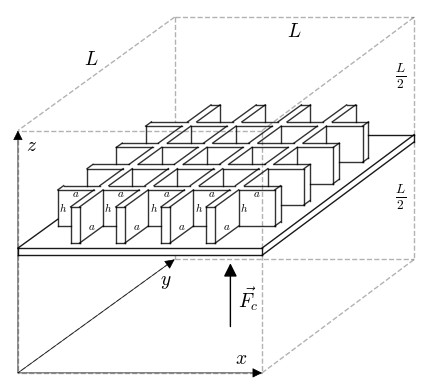
\includegraphics[width=0.48\textwidth]{honeycomb_box_L.png}
\caption{}{Cubic cavity with a plate \\ covered by honeycomb}
\end{center}
\label{fig:honeycomb_box_L}
\end{wrapfigure}

    \section{Two dimensional Casimir's
approach}\label{two-dimensional-casimirs-approach}

    Let us consider a cubic cavity of volume \(L^3\) bounded by perfectly
conducting walls and let a perfectly conducting square plate with side
\(L\) be placed in this cavity parallel to the \(xy\) face and let us
imagine the situation in which this plate is at a very large, say
\(L/2\) distance a from the \(xy\) face.

One side of this perfectly conducting square plate is a pure plane and
other is covered with perfectly conducting square-shaped honeycombs with
a square side \(a\).

On both sides of the the plate expressions \(\sum\hbar\omega\big/2\)
where the summation extends over all possible resonance frequencies of
the cavity \(L/2 \times L \times L\) (large cavity: beetween pure plane
and \(xy\) face) and the cavity \(L/2 \times a\times a\) (a small
cavity, one honeycomb cell: between the bottom of the honeycomb and the
opposite \(xy\) face) are divergent and devoid of physical meaning but
the difference between these sums on the opposite sides of the plate,
\(\left(\sum\,\,\hbar\omega\right)_{I}\big/{\left(2\,V_{I}\right)} - \left(\sum\,\,\hbar\omega\right)_{II}\big/{\left(2\,V_{II}\right)}\),
will be shown to have a well defined value and this value will be
interpreted as the interaction between the plate and the both remote
\(xy\) faces.

    The possible vibrations inside cavities defined by

    \(0<=x<=L\), \(0<=y<=L\), \(0<=z<=L/2\) (large cavity beetween pure
plane and \(xy\) face)

    and

    \(0<=x<=a\), \(0<=y<=a\), \(0<=z<=L/2\) (small cavity, one honeycomb
cell)

    have wave vectors

    \(k_x = \frac{\pi}{L}\,n_x\), \(k_y = \frac{\pi}{L}\,n_y\),
\(k_z = \frac{\pi}{L/2}\,n_z\) (large cavity beetween pure plane and
\(xy\) face),

    and

    \(k_x = \frac{\pi}{a}\,n_x\), \(k_y = \frac{\pi}{a}\,n_y\),
\(k_z = \frac{\pi}{L/2}\,n_z\) (small cavity, one honeycomb cell),

where \(n_x\). \(n_y\), \(n_z\) are positive integers;

    \(k = \sqrt{k_x^2+k_y^2+k_z^2} = \sqrt{\kappa^2+k_z^2}\).

    \(E = \frac{1}{2}\sum\,\hbar\omega = \hbar\,c\frac{1}{2}\sum\limits_{n_x}^{}\sum\limits_{n_y}^{}\sum\limits_{n_z}^{}k\)

    To every \(k_x\), \(k_y\), \(k_z\) correspond two standing waves unless
one of the \(n_i\) is zero, when there is only one.

    In case of one honeycomb cell cavity for \(k_z\) this is without
importance since for very large \(L/2\) we may regard \(k_z\) as
continuous variable, replacing summation over \(n_z\) with integration.
Thus we find

    \(\frac{1}{2}\sum\,\hbar\omega = \hbar\,c\frac{1}{2}\int\limits_{0}^{\infty}\left[{\sqrt{k_z^2}+2\sum\limits_{n_x=1}^{\infty}\sum\limits_{n_y=1}^{\infty}\sqrt{n_x^2\frac{\pi^2}{a^2}+n_y^2\frac{\pi^2}{a^2}+k_z^2}}\right]d{n_z}\)
(small cavity, one honeycomb cell),

    \(dn_z = \frac{L/2}{\pi}\,dk_z\),

    Now we can find the specific energy density \(E/V\), where
\(V = V_{small} = a^2 L/2\):

    \(\frac{1}{2\,V}\sum\,\hbar\omega = \frac{\hbar\,c}{a^2\,L/2}\frac{1}{2}\int\limits_{0}^{\infty}\left[{\sqrt{k_z^2}+2\sum\limits_{n_x=1}^{\infty}\sum\limits_{n_y=1}^{\infty}\sqrt{n_x^2\frac{\pi^2}{a^2}+n_y^2\frac{\pi^2}{a^2}+k_z^2}}\right]\frac{L/2}{\pi}\,dk_z\)
(small cavity, one honeycomb cell),

    \(\frac{1}{2\,V}\sum\,\hbar\omega = \frac{\hbar\,c}{a^2\,\pi}\int\limits_{0}^{\infty}\left[{\frac{1}{2}\sqrt{k_z^2}+\sum\limits_{n_x=1}^{\infty}\sum\limits_{n_y=1}^{\infty}\sqrt{n_x^2\frac{\pi^2}{a^2}+n_y^2\frac{\pi^2}{a^2}+k_z^2}}\right]\,dk_z\)
(small cavity, one honeycomb cell),

    \(\frac{1}{2\,V}\sum\,\hbar\omega = \frac{\hbar\,c}{a^2\,\pi}\int\limits_{0}^{\infty}\left[{\sum\limits_{n_x=(0)1}^{\infty}\sum\limits_{n_y=(0)1}^{\infty}\sqrt{n_x^2\frac{\pi^2}{a^2}+n_y^2\frac{\pi^2}{a^2}+k_z^2}}\right]\,dk_z\)
(small cavity, one honeycomb cell),

    where the notation \(\left(0\right) 1\) is meant to indicate that the
term with \(n_x = 0\) and \(n_y = 0\) has to be multiplied by
\(1\big/2\).

    \(\frac{1}{2\,V}\sum\,\hbar\omega = \frac{\hbar\,c}{a^2\,\pi}\sum\limits_{n_x=(0)1}^{\infty}\sum\limits_{n_y=(0)1}^{\infty}\left[\int\limits_{0}^{\infty}\sqrt{n_x^2\frac{\pi^2}{a^2}+n_y^2\frac{\pi^2}{a^2}+k_z^2}\,dk_z\right]\)
(small cavity, one honeycomb cell),

    And in case of large cavity for \(k_x\), \(k_y\) this is without
importance since for very large \(L\) we may regard \(k_x\), \(k_y\) as
continuous variables. Thus we find

    \(\frac{1}{2}\sum\,\hbar\omega = \hbar\,c\frac{1}{2}\int\limits_{0}^{\infty}\int\limits_{0}^{\infty}\left[{\sqrt{k_x^2+k_y^2}+2\sum\limits_{n_z=1}^{\infty}\sqrt{n_z^2\frac{\pi^2}{(L/2)^2}+k_x^2+k_y^2}}\right]d{n_x}d{n_y}\)
(large cavity beetween pure plane and \(xy\) face),

    For very large \(L/2\) also this last summation may be replaced by an
integral and it is therefore easily seen that energy is given by

    \(\frac{1}{2}\sum\,\hbar\omega = \hbar\,c\int\limits_{0}^{\infty}\int\limits_{0}^{\infty}\int\limits_{0}^{\infty}\sqrt{k_z^2+k_x^2+k_y^2}\,d{n_x}\,d{n_y}\,d{n_z}\)
(large cavity beetween pure plane and \(xy\) face),

    \(dn_x = \frac{L}{\pi}\,dk_x\), \(dn_y = \frac{L}{\pi}\,dk_y\),
\(dn_z = \frac{L/2}{\pi}\,dk_z\),

    Now we can find the specific energy density \(E/V\), where
\(V = V_{large} = L^3/2\) :

    \(\frac{1}{2\,V}\sum\,\hbar\omega = \frac{\hbar\,c}{L^3/2}\int\limits_{0}^{\infty}\int\limits_{0}^{\infty}\int\limits_{0}^{\infty}\sqrt{k_z^2+k_x^2+k_y^2}\,dn_x\,dn_y\,\frac{L/2}{\pi}\,dk_z\)
(large cavity beetween pure plane and \(xy\) face),

    \(\frac{1}{2\,V}\sum\,\hbar\omega = \frac{\hbar\,c}{L^2\,\pi}\int\limits_{0}^{\infty}\int\limits_{0}^{\infty}\left[\,\int\limits_{0}^{\infty}\sqrt{k_z^2+k_x^2+k_y^2}\,dk_z\right]\,dn_x\,dn_y\)
(large cavity beetween pure plane and \(xy\) face),

    \(\frac{1}{2\,V}\sum\,\hbar\omega = \frac{\hbar\,c}{L^2\,\pi}\int\limits_{0}^{\infty}\int\limits_{0}^{\infty}\left[\,\int\limits_{0}^{\infty}\sqrt{k_x^2+k_y^2+k_z^2}\,dk_z\right]\,dn_x\,dn_y\)
(large cavity beetween pure plane and \(xy\) face),

    \(\frac{1}{2\,V}\sum\,\hbar\omega = \frac{\hbar\,c}{L^2\,\pi}\int\limits_{0}^{\infty}\int\limits_{0}^{\infty}\left[\,\int\limits_{0}^{\infty}\sqrt{k_x^2+k_y^2+k_z^2}\,dk_z\right]\,\left(\frac{L}{\pi}dk_x\right)\,\left(\frac{L}{\pi}dk_y\right)\)
(large cavity beetween pure plane and \(xy\) face),

    \(\frac{1}{2\,V}\sum\,\hbar\omega = \frac{\hbar\,c}{a^2\,\pi}\int\limits_{0}^{\infty}\int\limits_{0}^{\infty}\left[\,\int\limits_{0}^{\infty}\sqrt{k_x^2+k_y^2+k_z^2}\,dk_z\right]\,\left(\frac{a}{\pi}dk_x\right)\,\left(\frac{a}{\pi}dk_y\right)\)
(large cavity beetween pure plane and \(xy\) face),

    \(\frac{1}{2\,V}\sum\,\hbar\omega = \frac{\hbar\,c}{a^2\,\pi}\sum\limits_{n_x=(0)1}^{\infty}\sum\limits_{n_y=(0)1}^{\infty}\left[\,\int\limits_{0}^{\infty}\sqrt{n_x^2\frac{\pi^2}{a^2}+n_y^2\frac{\pi^2}{a^2}+k_z^2}\,dk_z\right]\)
(small cavity, one honeycomb cell),

    it is therefore easily seen that our interaction energy is given by

    \[\begin{array}{lr}
\delta\,\frac{E}{V} =
\begin{array}{c}
\frac{\hbar\,c}{a^2\,\pi}\Bigg\{\sum\limits_{n_x=(0)1}^{\infty}\sum\limits_{n_y=(0)1}^{\infty}\left[\,\int\limits_{0}^{\infty}\sqrt{n_x^2\frac{\pi^2}{a^2}+n_y^2\frac{\pi^2}{a^2}+k_z^2}\,dk_z\right] - \\
\int\limits_{0}^{\infty}\int\limits_{0}^{\infty}\left[\,\int\limits_{0}^{\infty}\sqrt{k_x^2+k_y^2+k_z^2}\,dk_z\right]\,\left(\frac{a}{\pi}dk_x\right)\,\left(\frac{a}{\pi}dk_y\right)\Bigg\}
\end{array}\end{array}\]

    \[\begin{array}{lr}
\delta\,\frac{E}{V} =
\begin{array}{c}
\frac{\hbar\,c}{a^2\,\pi}\Bigg\{\sum\limits_{n_x=(0)1}^{\infty}\sum\limits_{n_y=(0)1}^{\infty}\left[\,\int\limits_{0}^{\infty}\sqrt{n_x^2\frac{\pi^2}{a^2}+n_y^2\frac{\pi^2}{a^2}+k_z^2}\,dk_z\right] - \\ \int\limits_{0}^{\infty}\int\limits_{0}^{\infty}\left[\,\int\limits_{0}^{\infty}\sqrt{k_x^2+k_y^2+k_z^2}\,dk_z\right]\,dn_x\,dn_y\Bigg\}
\end{array}\end{array}\]

    

    \({\left(\frac{E}{V}\right)_{small\,cavity} = \frac{1}{a^2}\,\hbar \, \sum\limits_{n_x=(0)1}^{\infty}\sum\limits_{n_y=(0)1}^{\infty}\,\int\limits_{0}^{\infty} {\frac {dk_{z}}{\pi}}\,\omega _{n_x,n_y},}\)

    where
\(\omega _{n_x,n_y} = c\,\sqrt{n_x^2\frac{\pi^2}{a^2}+n_y^2\frac{\pi^2}{a^2}+k_z^2}\)

    This expression is clearly infinite, and to proceed with the
calculation, it is convenient to introduce a regulator.

    In order to obtain a finite result it is necessary to multiply the
integrands by a regularization function \(f(k/k_m)\) which is unity for
\(k << k_m\) but tends to zero sufficiently rapidly for
\((k/k_m)\, \rightarrow\,\infty\). Where \(k_m\) may be defined by
\(f(1) = {1}/{2}\). The physical meaning is obvious: for very short
waves (X\textasciitilde{}rays e.g.) our plate is hardly an obstacle at
all and therefore the zero point energy of these waves will not be
influenced by the position of this plate.

    The regulator will serve to make the expression finite, and in the end
influence of its specific type will be removed by a limit transition.

    Introducing the variable \(u^2 = a^2\,k_z^2/\pi^2\),
\(du = a/\pi\,dk_z\), we have:

    \begin{equation}
\begin{array}{lr}
\delta\,\frac{E}{V} =
\begin{array}{c}
\frac{\hbar\,c\,\pi}{a^4}\Bigg\{
\sum\limits_{n_x=\left(0\right)\,1}^{\infty}
\sum\limits_{n_y=\left(0\right)\,1}^{\infty}
\int\limits_{0}^{\infty}
{\sqrt{n_x^2 + n_y^2 + u^2}}
f\left(\frac{\pi\sqrt{n_x^2 + n_y^2 + u^2}}{a\,k_m}\right)
\,d{u} \\
- \int\limits_{0}^{\infty}
\int\limits_{0}^{\infty}
\int\limits_{0}^{\infty}
{\sqrt{n_x^2 + n_y^2 + u^2}}
f\left(\frac{\pi\sqrt{n_x^2 + n_y^2 + u^2}}{a\,k_m}\right)
\,d{u}\,d{n_x}\,d{n_y}
\Bigg\}
\end{array}
\end{array}
\end{equation}

    If
\(\omega _{n_x,n_y} = c\,\sqrt{n_x^2\frac{\pi^2}{a^2}+n_y^2\frac{\pi^2}{a^2}+k_z^2}\)
and \(k_z^2 = u^2 \frac{\pi^2}{a^2}\) we have
\(\omega _{n_x,n_y} = c \, \frac{\pi}{a} \sqrt{n_x^2+n_y^2+u^2}\) so
\(f\left(\frac{\pi\sqrt{n_x^2 + n_y^2+u^2}}{a\,k_m}\right) = f\left(\frac{\omega _{n_x,n_y}}{c\,k_m}\right)\)
where the cutting frequency is \(\omega_m = c\,k_m\)

    Introducing function:

    \begin{equation}
F\left(u, n_x, n_y\right) = 
\sqrt{n_x^2 + n_y^2+u^2}\,
f\left(\frac{\pi\sqrt{n_x^2 + n_y^2+u^2}}{a\,k_m}\right)
\end{equation}

    we can write:

    \begin{equation}
\begin{array}{lr}
\delta\,\frac{E}{V} =
\begin{array}{c}
\frac{\hbar\,c\,\pi}{a^4}
\Bigg\{
\sum\limits_{n_x=\left(0\right)\,1}^{\infty}
\sum\limits_{n_y=\left(0\right)\,1}^{\infty}
\left(\int\limits_{0}^{\infty}F\left(u, n_x, n_y\right)\,d{u}\right)
- \\
\int\limits_{0}^{\infty}
\int\limits_{0}^{\infty}
\left(\int\limits_{0}^{\infty}F\left(u, n_x, n_y\right)\,d{u}\right)
\,d{n_x}\,d{n_y}
\Bigg\}
\end{array}
\end{array}
\end{equation}

    And at least, introducing

    \begin{equation}
G\left(n_x, n_y\right) = \int\limits_{0}^{\infty}F\left(u, n_x, n_y\right)\,d{u}
\end{equation}

    We have

    \begin{equation}
\delta\,\frac{E}{V} = \frac{\hbar\,c\,\pi}{a^4}
\left\{
\sum\limits_{n_x=\left(0\right)\,1}^{\infty}
\sum\limits_{n_y=\left(0\right)\,1}^{\infty}
G\left(n_x, n_y\right)
-
\int\limits_{0}^{\infty}
\int\limits_{0}^{\infty}
G\left(n_x, n_y\right)
\,d{n_x}\,d{n_y}
\right\}
\end{equation}

Integration of \(G\left(n_x, n_y\right)\) with example of regulator
function see in Appendix A.

    Now aiming to receive a way of calculating \(\delta\left(E/V\right)\) we
should consider

\section{Euler--Maclaurin 2D formula}\label{eulermaclaurin-2d-formula}

According to A.Bikyalis \cite{Bikyalis1968} we just apply Euler -
Maclaurin formula twice on \(n_x\) and on \(n_y\)

Starting from the following form of this formula

\[{\displaystyle \sum _{i=a}^{b}f(i)=\int _{a}^{b}f(x)\,dx+{\frac {f(a)+f(b)}{2}}+\sum _{k=1}^{\lfloor p/2\rfloor }{\frac {B_{2k}}{(2k)!}}\left(f^{(2k-1)}(b)-f^{(2k-1)}(a)\right)+R_{p},}\]

\[{\displaystyle P_{k}(x)=B_{k}\left(x-\lfloor x\rfloor \right),}\]

\[{\displaystyle R_{p}=(-1)^{p+1}\int _{a}^{b}f^{(p)}(x){\frac {P_{p}(x)}{p!}}\,dx.}\]

or better since we are dealing with a mathematically very complex
problem of integration that is rather difficult, often oscillating and
suffering discontinuities at the points of each integer value of the
argument due to the presence of the multiplier \((x-\lfloor x\rfloor )\)
of the function, we will use the fact that the remainder term can also
be expressed in the form:

\[{\displaystyle R_{p}=(-1)^{p+1}\sum_{j=a}^{b-1} \int _{0}^{1}f^{(p)}(v+j){\frac {B_{p}(v)}{p!}}\,dv.}\]

we see that it consists of 4 terms:

integral \(\int\limits_{x}^{}=\int _{x_a}^{x_b}f(x)\,dx\),

half sum \(\underset{x}{H_{\sum}}={\left( {f(x_a)+f(x_b)}\right)/{2}}\),

sum of Bernoulli polynomials
\({\sum\limits_{x}^{}}^{B}=\sum _{k=1}^{\lfloor p/2\rfloor }{\frac {B_{2k}}{(2k)!}}\left(f^{(2k-1)}(x_b)-f^{(2k-1)}(x_a)\right)\)

and the remainder term
\(\underset{x}{R_{p}}=(-1)^{p+1}\sum_{j=x_a}^{x_b-1} \int _{0}^{1}f^{(p)}(v_x+j_x){\frac {B_{p}(v_x)}{p!}}\,dv_x\).

When applying it to \(G\) twice on \(n_x\) and on \(n_y\) we should have
the following terms which can be represented in the table form:

    \begin{equation}
\begin{array}{cccc}
 \int\limits_{n_y}^{} \int\limits_{n_x}^{} G  &  \int\limits_{n_y}^{} \underset{n_x}{H_{\sum}}\,G  &  \int\limits_{n_y}^{}{\sum\limits_{n_x}^{}}^{B}\,G  &  \int\limits_{n_y}^{}\,\underset{n_x}{R_{p}}\,G  \\
 \underset{n_y}{H_{\sum}}\,\int\limits_{n_x}^{}\,G &  \underset{n_y}{H_{\sum}}\,\underset{n_x}{H_{\sum}}\,G &  \underset{n_y}{H_{\sum}}\,{\sum\limits_{n_x}^{}}^{B}\,G &  \underset{n_y}{H_{\sum}}\,\underset{n_x}{R_{p}}\,G \\
 {\sum\limits_{n_y}^{}}^{B}\,\int\limits_{n_x}^{}\,G  &  {\sum\limits_{n_y}^{}}^{B}\,\underset{n_x}{H_{\sum}}\,G  &  {\sum\limits_{n_y}^{}}^{B}\,{\sum\limits_{n_x}^{}}^{B}\,G  &  {\sum\limits_{n_y}^{}}^{B}\,\underset{n_x}{R_{p}}\,G  \\
 \underset{n_y}{R_{p}}\,\int\limits_{n_x}^{}\,G   &  \underset{n_y}{R_{p}}\,\underset{n_x}{H_{\sum}}\,G   &  \underset{n_y}{R_{p}}\,{\sum\limits_{n_x}^{}}^{B}\,G   &  \underset{n_y}{R_{p}}\,\underset{n_x}{R_{p}}\,G
\end{array}\end{equation}

    And taking on account that we have function \(G\) which is symmetric on
its \(n_x\) and \(n_y\) arguments, so above two dimentional
Euler--Maclaurin marix is symmetric too.

    \section{Summary of Euler--Maclaurin
2D}\label{summary-of-eulermaclaurin-2d}

Taking value of parameter \(p = 1\) we have:

    \begin{center}
\begin{tabular}{ | l | }
\hline

$\int\limits_{n_y}^{} \int\limits_{n_x}^{} G = \int_{a_{y}}^{b_{y}} \int_{a_{x}}^{b_{x}} G\left(n_{x}, n_{y}\right)\,{d n_{x}}\,{d n_{y}}$ \\

$\int\limits_{n_y}^{} \underset{n_x}{H_{\sum}}\,G = \frac{1}{2} \, \int_{a_{y}}^{b_{y}} G\left(a_{x}, n_{y}\right)\,{d n_{y}}$ \\

$\int\limits_{n_y}^{} {\sum\limits_{n_x}^{}}^{B}\,G = 0$ \\

$\int\limits_{n_y}^{} \underset{n_x}{R_{p}}\,G = {\sum_{j_{x}=a_{x}}^{b_{x} - 1} \int_{a_{y}}^{b_{y}} \int_{0}^{1} \frac{1}{2} \, {\left(2 \, v_{n_{x}} - 1\right)} \mathrm{D}_{0}\left(G\right)\left(j_{x} + v_{n_{x}}, n_{y}\right)\,{d v_{n_{x}}}\,{d n_{y}}}$ \\

\hline\hline

$\underset{n_y}{H_{\sum}}\,\int\limits_{n_x}^{}\,G = \frac{1}{2} \, \int_{a_{x}}^{b_{x}} G\left(n_{x}, a_{y}\right)\,{d n_{x}}$ \\

$\underset{n_y}{H_{\sum}}\,\underset{n_x}{H_{\sum}}\,G = \frac{1}{4} \, G\left(a_{x}, a_{y}\right)$ \\

$\underset{n_y}{H_{\sum}}\,{\sum\limits_{n_x}^{}}^{B}\,G = 0$ \\

$\underset{n_y}{H_{\sum}}\,\underset{n_x}{R_{p}}\,G = {\sum_{j_{n_{x}}=a_{x}}^{b_{x} - 1} \frac{1}{4} \, \int_{0}^{1} \left(2 \, v_{n_{x}} - 1 \right) \mathrm{D}_{0}\left(G\right)\left(j_{n_{x}} + v_{n_{x}}, a_{y}\right)\,{d v_{n_{x}}} }$ \\

\hline\hline

${\sum\limits_{n_y}^{}}^{B}\,\int\limits_{n_x}^{}\,G = 0$ \\

${\sum\limits_{n_y}^{}}^{B}\,\underset{n_x}{H_{\sum}}\,G = 0$ \\

${\sum\limits_{n_y}^{}}^{B}\,{\sum\limits_{n_x}^{}}^{B}\,G = 0$ \\

${\sum\limits_{n_y}^{}}^{B}\,\underset{n_x}{R_{p}}\,G = 0$ \\

\hline\hline

$\underset{n_y}{R_{p}}\,\int\limits_{n_x}^{}\,G = {\sum_{j_{x}=a_{x}}^{b_{x} - 1} \int_{a_{y}}^{b_{y}} \int_{0}^{1} \frac{1}{2} \, {\left(2 \, v_{n_{x}} - 1\right)} \mathrm{D}_{0}\left(G\right)\left(j_{x} + v_{n_{x}}, n_{y}\right)\,{d v_{n_{x}}}\,{d n_{y}}}$ \\

$\underset{n_y}{R_{p}}\,\underset{n_x}{H_{\sum}}\,G = {\sum_{j_{n_{y}}=a_{y}}^{b_{y} - 1} \int_{0}^{1} \frac{1}{4} \, {\left(2 \, v_{n_{y}} - 1\right)} \mathrm{D}_{1}\left(G\right)\left(a_{x}, j_{n_{y}} + v_{n_{y}}\right)\,{d v_{n_{y}}}}$ \\

$\underset{n_y}{R_{p}}\,{\sum\limits_{n_x}^{}}^{B}\,G = 0$ \\

$\underset{n_y}{R_{p}}\,\underset{n_x}{R_{p}}\,G = {\sum_{j_{y}=a_{y}}^{b_{y} - 1} {\sum_{j_{x}=a_{x}}^{b_{x} - 1} \int_{0}^{1} \int_{0}^{1}\frac{1}{4} \, {\left(2 \, v_{y} - 1\right)}  {\left(2 \, v_{x} - 1\right)} \mathrm{D}_{0, 1}\left(G\right)\left(j_{x} + v_{x}, j_{y} + v_{y}\right)\,{d v_{x}}}\,{d v_{y}}}$ \\

\hline

\end{tabular}
\end{center}

    \section{\texorpdfstring{A way of calculating
\(\delta\left(E/V\right)\)}{A way of calculating \textbackslash{}delta\textbackslash{}left(E/V\textbackslash{}right)}}\label{a-way-of-calculating-deltaleftevright}

    Let's consider

\[
\sum\limits_{n_x=\left(0\right)\,1}^{\infty}
\sum\limits_{n_y=\left(0\right)\,1}^{\infty}
G\left(n_x, n_y\right)
-
\int\limits_{0}^{\infty}
\int\limits_{0}^{\infty}
G\left(n_x, n_y\right)\,d{n_x}\,d{n_y}
\]

    First we see, that

    \(\sum\limits_{n_x=\left(0\right)\,1}^{\infty} \sum\limits_{n_y=\left(0\right)\,1}^{\infty} {G\left(n_x, n_y\right)} = \\ \sum\limits_{n_x=\left(0\right)\,1}^{\infty} \left( -\frac{1}{2}G\left(n_x, 0\right) + \sum\limits_{n_y=0}^{\infty}{G\left(n_x, n_y\right)} \right) = \\ -\frac{1}{2} \left( -\frac{1}{2}G\left(0, 0\right) + \sum\limits_{n_y=0}^{\infty}{G\left(0, n_y\right)} \right) +\sum\limits_{n_x=0}^{\infty} \left( -\frac{1}{2}G\left(n_x, 0\right) + \sum\limits_{n_y=0}^{\infty}{G\left(n_x, n_y\right)} \right) = \\ \frac{1}{4}G\left(0, 0\right) - \frac{1}{2}\sum\limits_{n_y=0}^{\infty}{G\left(0, n_y\right)} - \frac{1}{2}\sum\limits_{n_x=0}^{\infty}{G\left(n_x, 0\right)} + \sum\limits_{n_x=0}^{\infty}\sum\limits_{n_y=0}^{\infty}{G\left(n_x, n_y\right)}\)

    So we have

\(\sum\limits_{n_x=\left(0\right)\,1}^{\infty} \sum\limits_{n_y=\left(0\right)\,1}^{\infty} G\left(n_x, n_y\right) - \int\limits_{0}^{\infty} \int\limits_{0}^{\infty} G\left(n_x, n_y\right)\,d{n_x}\,d{n_y} = \\ \frac{1}{4}G\left(0, 0\right) -\frac{1}{2}\sum\limits_{n_y=0}^{\infty}{G\left(0, n_y\right)} -\frac{1}{2}\sum\limits_{n_x=0}^{\infty}{G\left(n_x, 0\right)} +\sum\limits_{n_x=0}^{\infty}\sum\limits_{n_y=0}^{\infty}{G\left(n_x, n_y\right)} - \int\limits_{0}^{\infty} \int\limits_{0}^{\infty} G\left(n_x, n_y\right)\,d{n_x}\,d{n_y}\)

    On the other hand we have found that

\(\sum\limits_{n_x=0}^{\infty} \sum\limits_{n_y=0}^{\infty} G\left(n_x, n_y\right) -\int\limits_{0}^{\infty} \int\limits_{0}^{\infty} G\left(n_x, n_y\right)\,d{n_x}\,d{n_y} = \\ \begin{array}{cccc}  \, &  \int\limits_{n_y}^{} \underset{n_x}{H_{\sum}}\,G &  + \int\limits_{n_y}^{}{\sum\limits_{n_x}^{}}^{B}\,G &  + \int\limits_{n_y}^{}\,\underset{n_x}{R_{p}}\,G \\  +\underset{n_y}{H_{\sum}}\,\int\limits_{n_x}^{}\,G &  + \underset{n_y}{H_{\sum}}\,\underset{n_x}{H_{\sum}}\,G &  + \underset{n_y}{H_{\sum}}\,{\sum\limits_{n_x}^{}}^{B}\,G &  + \underset{n_y}{H_{\sum}}\,\underset{n_x}{R_{p}}\,G \\  + {\sum\limits_{n_y}^{}}^{B}\,\int\limits_{n_x}^{}\,G &  + {\sum\limits_{n_y}^{}}^{B}\,\underset{n_x}{H_{\sum}}\,G &  + {\sum\limits_{n_y}^{}}^{B}\,{\sum\limits_{n_x}^{}}^{B}\,G &  + {\sum\limits_{n_y}^{}}^{B}\,\underset{n_x}{R_{p}}\,G \\  + \underset{n_y}{R_{p}}\,\int\limits_{n_x}^{}\,G &  + \underset{n_y}{R_{p}}\,\underset{n_x}{H_{\sum}}\,G &  + \underset{n_y}{R_{p}}\,{\sum\limits_{n_x}^{}}^{B}\,G &  + \underset{n_y}{R_{p}}\,\underset{n_x}{R_{p}}\,G \end{array}\)

    where \(\underset{n_y}{H_{\sum}}\,\underset{n_x}{H_{\sum}}\,G\),
\(\int\limits_{n_y}^{} \underset{n_x}{H_{\sum}}\,G\) and
\(\underset{n_y}{H_{\sum}}\,\int\limits_{n_x}^{}\,G\) are:

    \(\frac{1}{4} \, G\left(a_{x}, a_{y}\right) , \frac{1}{2} \, \int_{a_{y}}^{b_{y}} G\left(a_{x}, n_{y}\right)\,{d n_{y}} , \frac{1}{2} \, \int_{a_{x}}^{b_{x}} G\left(n_{x}, a_{y}\right)\,{d n_{x}}\)

    Now using 1D Euler--Maclaurin formula in form:

    \[{\displaystyle \sum _{i=a}^{b}f(i)=\int _{a}^{b}f(x)\,dx+{\frac {f(a)+f(b)}{2}}+\sum _{k=1}^{\lfloor p/2\rfloor }{\frac {B_{2k}}{(2k)!}}(f^{(2k-1)}(b)-f^{(2k-1)}(a))+R_{p},}\]

    we can see that

    \[
\frac{1}{4}G\left(0, 0\right)
- \frac{1}{2}\sum\limits_{n_y=0}^{\infty}{G\left(0, n_y\right)}
- \frac{1}{2}\sum\limits_{n_x=0}^{\infty}{G\left(n_x, 0\right)}
\]

    will be equal to

    \(\begin{array}{rrllll}  \underset{n_y}{H_{\sum}}\,\underset{n_x}{H_{\sum}}\,G \\  \, &  - \int\limits_{n_y}^{} \underset{n_x}{H_{\sum}}\,G &  - \underset{n_y}{H_{\sum}} \underset{n_x}{H_{\sum}}\,G &  - \frac{1}{2}{\sum\limits_{n_y}^{}}^{B}\,G &  - \frac{1}{2}\underset{n_y}{R_{p}}\,G/2 \\  \,&  - \underset{n_y}{H_{\sum}}\int\limits_{n_x}^{} \,G &  - \underset{n_y}{H_{\sum}} \underset{n_x}{H_{\sum}}\,G &  - \frac{1}{2}{\sum\limits_{n_x}^{}}^{B}\,G &  - \frac{1}{2}\underset{n_x}{R_{p}}\,G/2 \\ \end{array}\)

    So we can find

\(\sum\limits_{n_x=\left(0\right)\,1}^{\infty} \sum\limits_{n_y=\left(0\right)\,1}^{\infty} G\left(n_x, n_y\right) - \int\limits_{0}^{\infty} \int\limits_{0}^{\infty} G\left(n_x, n_y\right)\,d{n_x}\,d{n_y}\)

using the following formula:

    \(\begin{array}{llll}  \,&  \,&  + \int\limits_{n_y}^{}{\sum\limits_{n_x}^{}}^{B}\,G &  + \int\limits_{n_y}^{}\,\underset{n_x}{R_{p}}\,G \\  \,&  \,&  + \underset{n_y}{H_{\sum}}\,{\sum\limits_{n_x}^{}}^{B}\,G &  + \underset{n_y}{H_{\sum}}\,\underset{n_x}{R_{p}}\,G \\  + {\sum\limits_{n_y}^{}}^{B}\,\int\limits_{n_x}^{}\,G &  + {\sum\limits_{n_y}^{}}^{B}\,\underset{n_x}{H_{\sum}}\,G &  + {\sum\limits_{n_y}^{}}^{B}\,{\sum\limits_{n_x}^{}}^{B}\,G &  + {\sum\limits_{n_y}^{}}^{B}\,\underset{n_x}{R_{p}}\,G \\  + \underset{n_y}{R_{p}}\,\int\limits_{n_x}^{}\,G &  + \underset{n_y}{R_{p}}\,\underset{n_x}{H_{\sum}}\,G &  + \underset{n_y}{R_{p}}\,{\sum\limits_{n_x}^{}}^{B}\,G &  + \underset{n_y}{R_{p}}\,\underset{n_x}{R_{p}}\,G \\  \,&  \,&  - \frac{1}{2}{\sum\limits_{n_y}^{}}^{B}\,G &  - \frac{1}{2}\underset{n_y}{R_{p}}\,G \\  \,&  \,&  - \frac{1}{2}{\sum\limits_{n_x}^{}}^{B}\,G &  - \frac{1}{2}\underset{n_x}{R_{p}}\,G \\ \end{array}\)

    It is easy to see that all terms without remainder part:

    \(\begin{array}{llll}  \,&  \,&  + \int\limits_{n_y}^{}{\sum\limits_{n_x}^{}}^{B}\,G \\  \,&  \,&  + \underset{n_y}{H_{\sum}}\,{\sum\limits_{n_x}^{}}^{B}\,G \\  + {\sum\limits_{n_y}^{}}^{B}\,\int\limits_{n_x}^{}\,G &  + {\sum\limits_{n_y}^{}}^{B}\,\underset{n_x}{H_{\sum}}\,G &  + {\sum\limits_{n_y}^{}}^{B}\,{\sum\limits_{n_x}^{}}^{B}\,G\\  \,&  \,&  - \frac{1}{2}{\sum\limits_{n_y}^{}}^{B}\,G \\  \,&  \,&  - \frac{1}{2}{\sum\limits_{n_x}^{}}^{B}\,G \\ \end{array}\)

    are 0 in sum. And so any possible non zero result should be related with
remainder part:

    \(\begin{array}{r} \sum\limits_{n_x=\left(0\right)\,1}^{\infty} \sum\limits_{n_y=\left(0\right)\,1}^{\infty} G\left(n_x, n_y\right) - \int\limits_{0}^{\infty} \int\limits_{0}^{\infty} G\left(n_x, n_y\right)\,d{n_x}\,d{n_y} = \end{array}\)

    \(\begin{array}{llll}  \,&  \,&  \,&  + \int\limits_{n_y}^{}\,\underset{n_x}{R_{p}}\,G \\  \,&  \,&  \,&  + \underset{n_y}{H_{\sum}}\,\underset{n_x}{R_{p}}\,G \\  \,&  \,&  \,&  + {\sum\limits_{n_y}^{}}^{B}\,\underset{n_x}{R_{p}}\,G \\  + \underset{n_y}{R_{p}}\,\int\limits_{n_x}^{}\,G &  + \underset{n_y}{R_{p}}\,\underset{n_x}{H_{\sum}}\,G &  + \underset{n_y}{R_{p}}\,{\sum\limits_{n_x}^{}}^{B}\,G &  + \underset{n_y}{R_{p}}\,\underset{n_x}{R_{p}}\,G \\  \,&  \,&  \,&  - \frac{1}{2}\underset{n_y}{R_{p}}\,G \\  \,&  \,&  \,&  - \frac{1}{2}\underset{n_x}{R_{p}}\,G \\ \end{array}\)

    Or using symmetric properties of \(G\) we can rewrite result formula:

    \(\begin{array}{r} \sum\limits_{n_x=\left(0\right)\,1}^{\infty} \sum\limits_{n_y=\left(0\right)\,1}^{\infty} G\left(n_x, n_y\right) - \int\limits_{0}^{\infty} \int\limits_{0}^{\infty} G\left(n_x, n_y\right)\,d{n_x}\,d{n_y} = \end{array}\)

    \(+\,2\cdot\underset{n_y}{R_{p}}\,\int\limits_{n_x}^{}\,G +\,2\cdot\underset{n_y}{R_{p}}\,\underset{n_x}{H_{\sum}}\,G +\,2\cdot\underset{n_y}{R_{p}}\,{\sum\limits_{n_x}^{}}^{B}\,G +\,\underset{n_y}{R_{p}}\,\underset{n_x}{R_{p}}\,G -\,\underset{n_y}{R_{p}}\,G\)

    with the following terms:

\(2\cdot\underset{n_y}{R_{p}}\,\int\limits_{n_x}^{}\,G\left(u\right) = 2 \, {\sum\limits_{j_{x}=a_{x}}^{b_{x} - 1} \int\limits_{a_{y}}^{b_{y}} \int\limits_{0}^{1} \frac{1}{2} \, {\left(2 \, v_{n_{x}} - 1\right)} \mathrm{D}_{0}\left(G\right)\left(j_{x} + v_{n_{x}}, n_{y}\right)\,{d v_{n_{x}}}\,{d n_{y}}}\)

\(2\cdot\underset{n_y}{R_{p}}\,\underset{n_x}{H_{\sum}}\,G\left(u\right) = 2 \, {\sum\limits_{j_{n_{y}}=a_{y}}^{b_{y} - 1} \int\limits_{0}^{1} \frac{1}{4} \, {\left(2 \, v_{n_{y}} - 1\right)} \mathrm{D}_{1}\left(G\right)\left(a_{x}, j_{n_{y}} + v_{n_{y}}\right)\,{d v_{n_{y}}}}\)

\(2\cdot\underset{n_y}{R_{p}}\,{\sum\limits_{n_x}^{}}^{B}\,G\left(u\right) = 2 \, {\sum\limits_{j_{n_{y}}=a_{y}}^{b_{y} - 1} \int\limits_{0}^{1} 0\,{d v_{n_{y}}}}\)

\(\underset{n_y}{R_{p}}\,\underset{n_x}{R_{p}}\,G = {\sum\limits_{j_{y}=a_{y}}^{b_{y} - 1} {\sum\limits_{j_{x}=a_{x}}^{b_{x} - 1} \int\limits_{0}^{1} \int\limits_{0}^{1} \frac{1}{4} \, {\left(2 \, v_{y} - 1\right)} {\left(2 \, v_{x} - 1\right)} \mathrm{D}_{0, 1}\left(G\right)\left(j_{x} + v_{x}, j_{y} + v_{y}\right)\,{d v_{x}}}\,{d v_{y}}}\)

\(-\underset{n_y}{R_{p}}\,G = -{\sum\limits_{j_{n_{y}}=a_{y}}^{b_{y} - 1} \int\limits_{0}^{1} \frac{1}{2} \, {\left(2 \, v_{n_{y}} - 1\right)} \mathrm{D}_{1}\left(G\right)\left(n_{x}, j_{n_{y}} + v_{n_{y}}\right)\,{d v_{n_{y}}}}\)

    Considering \(\underset{n_y}{R_{p}}\,{\sum\limits_{n_x}^{}}^{B}\,G\)
should be \(0\), because derivative with respect to \(n_x\) when
\(n_x = 0\) gives \(0\), and
\(\,2\cdot\underset{n_y}{R_{p}}\,\underset{n_x}{H_{\sum}}\,G -\,\underset{n_y}{R_{p}}\,G\)
gives \(0\) in summation, we can simplify result in form:

    \begin{equation}
\begin{array}{r}
\sum\limits_{n_x=\left(0\right)\,1}^{\infty}
\sum\limits_{n_y=\left(0\right)\,1}^{\infty}
G\left(n_x, n_y\right)
-
\int\limits_{0}^{\infty}
\int\limits_{0}^{\infty}
G\left(n_x, n_y\right)\,d{n_x}\,d{n_y} =
\,2\cdot\underset{n_y}{R_{p}}\,\int\limits_{n_x}^{}\,G 
+\,\underset{n_y}{R_{p}}\,\underset{n_x}{R_{p}}\,G
\end{array}
\end{equation}

    or in detailed form:

\begin{equation}
\begin{array}{l}
\sum\limits_{n_x=\left(0\right)\,1}^{\infty}
\sum\limits_{n_y=\left(0\right)\,1}^{\infty}
G\left(n_x, n_y\right)
-
\int\limits_{0}^{\infty}
\int\limits_{0}^{\infty}
G\left(n_x, n_y\right)\,d{n_x}\,d{n_y} = \\
{\sum\limits_{j_{x}=0}^{\infty} \int\limits_{n_{y}=0}^{\infty} \int\limits_{v_x=0}^{1}  {\left(2 \, v_{n_{x}} - 1\right)} \mathrm{D}_{0}\left(G\right)\left(j_{x} + v_{n_{x}}, n_{y}\right)\,{d v_{n_{x}}}\,{d n_{y}}} + \\
\frac{1}{4} \, {\sum\limits_{j_{y}=0}^{\infty} {\sum\limits_{j_{x}=0}^{\infty} \int\limits_{0}^{1} \int\limits_{0}^{1} {\left(2 \, v_{y} - 1\right)} {\left(2 \, v_{x} - 1\right)} \mathrm{D}_{0, 1}\left(G\right)\left(j_{x} + v_{x}, j_{y} + v_{y}\right)\,{d v_{x}}}\,{d v_{y}}}
\end{array}
\end{equation}

    \section{\texorpdfstring{How \(\delta\left(E/V\right)\) depends on
\(a k_m\)
?}{How \textbackslash{}delta\textbackslash{}left(E/V\textbackslash{}right) depends on a k\_m ?}}\label{how-deltaleftevright-depends-on-a-k_m}

    Casimir in his original work has provided his formula in assumption when
as \(a\,k_m\,»\,1\). But now we can investigate how

\(\sum\limits_{n_x=\left(0\right)\,1}^{\infty} \sum\limits_{n_y=\left(0\right)\,1}^{\infty} G\left(n_x, n_y\right) - \int\limits_{0}^{\infty} \int\limits_{0}^{\infty} G\left(n_x, n_y\right)\,d{n_x}\,d{n_y}\)

will depends on \(a k_m\)

    \begin{center}
\begin{tabular}{ | l | c | c | c | }
\hline
$a \cdot k_m$ & $\sum\limits_{\left(0\right)\,1}^{\infty}\sum\limits_{\left(0\right)\,1}^{\infty}-\int\limits_{0}^{\infty}\int\limits_{0}^{\infty}G$ & $\epsilon$ & $j_{max}$ \\
\hline
0.25 & 0.0010898998026781217 & 4.996697073620143e-07 & 2 \\
0.5 & 0.0032237749029524953 & 7.998369526561223e-07 & 6 \\
0.75 & 0.004403922584267899 & 8.721734991096397e-07 & 11 \\
1.0 & 0.003048368039753142 & 8.495559555607291e-07 & 17 \\
1.25 & -0.0014811539004775248 & 1.7711588730298828e-06 & 18 \\
1.5 & -0.008708226320289525 & 3.6727148564415e-06 & 18 \\
1.75 & -0.01722786703218093 & 6.80405403998826e-06 & 18 \\
2.0 & -0.025174603512904688 & 9.989436530283013e-06 & 19 \\
2.25 & -0.030834142522710325 & 9.370330676246764e-06 & 23 \\
2.5 & -0.03328670643720081 & 1.4281938944775391e-05 & 23 \\
2.75 & -0.03243630208049284 & 2.091015549165456e-05 & 23 \\
3.0 & -0.028986396523536337 & 2.961508478431949e-05 & 23 \\
3.25 & -0.024047951283080123 & 4.0789713256873105e-05 & 23 \\
3.5 & -0.018309169743688476 & 8.561178612309775e-06 & 45 \\
3.75 & -0.013591792977477306 & 2.1853680230903085e-05 & 36 \\
4 & -0.009731507224089121 & 1.4610545561998458e-05 & 45 \\
4.5 & -0.006342700310733549 & 1.9329818693328873e-05 & 48 \\
5 & -0.007323343929996339 & 2.3242272627768528e-05 & 52 \\
6 & -0.012436017530558603 & 2.3732800946523056e-05 & 66 \\
7 & -0.014209420986523558 & 3.8533275062919475e-05 & 69 \\
8 & -0.0136610172109347 & 3.293747500025098e-05 & 87 \\
9 & -0.013782731174753638 & 3.585979757156756e-05 & 99 \\
\hline
\end{tabular}
\end{center}

    Thus for the energy density difference per \(cm^2\) we find

    \(\delta\,\frac{E}{V} = \frac{\hbar\,c\,\pi}{a^4} \int\limits_{0}^{\infty}{ \left\{ \sum\limits_{n_x=\left(0\right)\,1}^{\infty} \sum\limits_{n_y=\left(0\right)\,1}^{\infty} F\left(n_x, n_y\right) - \int\limits_{0}^{\infty} \int\limits_{0}^{\infty} F\left(n_x, n_y\right)\,d{n_x}\,d{n_y} \right\} }\,d{u}\)

    According to our calculation we can see that

    \(\int\limits_{0}^{\infty}{ \left\{ \sum\limits_{n_x=\left(0\right)\,1}^{\infty} \sum\limits_{n_y=\left(0\right)\,1}^{\infty} F\left(n_x, n_y\right) - \int\limits_{0}^{\infty} \int\limits_{0}^{\infty} F\left(n_x, n_y\right)\,d{n_x}\,d{n_y} \right\} }\,d{u} \approx R\left(a k_m\right)\)

    \begin{wrapfigure}{r}{0.5\textwidth}
\begin{center}
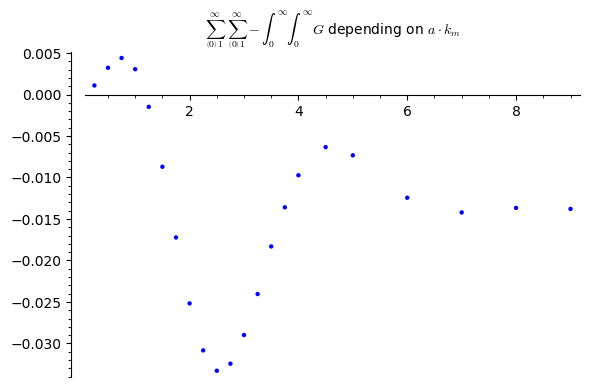
\includegraphics[width=0.48\textwidth]{sum_sum_int_int_G_on_a_km.png}
\caption{}{How $\delta\left(E/V\right)$ depends on $a k_m$}
\end{center}
\label{fig:G_on_a_km}
\end{wrapfigure}

    Where \(R\left(a k_m\right)\) is some function depended on material
properties with well defined limit at \(a\,k_m\,»\,1\). So

    \begin{equation}
\delta\,\frac{E}{V} = R\left(a k_m\right)\,\frac{\hbar\,c\,\pi}{a^4}
\end{equation}

    For the energy density difference per \(cm^2\) (in the limit as
\(a\,k_m\,\rightarrow \,10\)) we find

    \(\delta\,\frac{E}{V} = \hbar\,c\, \pi\frac{R}{a^4}\,=\,0.0136\,\frac{1}{a_{\mu}^4}\,dyne/cm^2\)

    where \(a_{\mu}\) is a square side of honeycombs measured in microns.

    Can this difference of specific energy density
\(\delta\left(E/V\right)\) be interpreted as the cause of the force
\(F\) applied to perfectly conducting honeycomb on a plate? For example
my investigations of the original Casimir's configuration shown that in
geometric configuration of two perfectly conducting plates
\(F/S = -3 \cdot \delta\left(E/V\right)\). But what about honeycomb
configutation? Investigation of this question in appendixes B and C
shows that \(F/S \approx \delta\left(E/V\right)\).

    \section{Conclusions}\label{conclusions}

    We are thus led to the following conclusions. There is a force applied
to perfectly conducting honeycombs on a plate as a result of the
difference in specific energy density on its different sides. This force
is dependent of the material of the plate. This force depends at least
on the cutoff frequency \(\omega_m\) of the honeycomb plate material.
This force can be interpreted as the pressure of the zero point
electromagnetic oscillations.

    Although the effect is small, an experimental confirmation seems not
unfeasable and might be of a certain interest.

    Tuo Qu, Fang Liu, Yuechai Lin, Yidong Huang \cite{Tuo2019} reported
about the production of gold nano-honeycomb with a size of about 2
microns.

According to the formula received in this work such honeycomb should
have the difference Casimir energy densities about
\(\delta\left(E/V\right) = 0.0136/({2^4}) = 0.0008555\,dyne/cm^2 = 0.0008555 \cdot 10^4 = 8.55\,dyne/m^2\),
that is 8.55 dynes per square meter of the panel, which is already quite
an acceptable value for the practical use of the expected effect for
correcting satellite orbits.

The only thing to point out is that, according to my method of
calculation, the resulting formula gives \(\delta\left(E/V\right)\)
calculated not for the total surface area of the honeycombs, but for
part of the panel's area occupied by recesses (minus the part of the
honeycomb area occupied by walls).

This does not mean the need to strive to make very thin walls of the
honeycomb, because with a decrease in the wall thickness, the value of
\(k_m\) will also decrease.

In addition, the weak point of my calculation is the implicit assumption
of the infinite value of the height of the walls of the honeycombs,
while the real height of the walls will be finite.

At the same time, using the Antipin approach (see Appendix D), it can be
shown that the effect should also be observed at a finite height of the
ribs, although the dependence of the effect on this height may be the
subject of further research.

The final actual height of the walls will make some correction to the
value of the result obtained (which may be a topic for further
research), but the fundamental conclusion will not change.

Regarding criticism: Hrvoje \cite{Hrvoje2016} consider the Casimir
effect not as a consequence of the existence of virtual quantum photons,
but as only a manifestation of the London-van der Waals dispersion
forces.

I want to note that setting up an experiment to measure the thrust force
produced by nanocells grown on metal could serve as a kind of critical
experiment to find out which of the points of view on the nature of the
Casimir forces corresponds to reality.

    \section{Appendix A. Integration
details}\label{appendix-a.-integration-details}

    Let's use the regularization function in the form

    \[f\left(\frac{k}{k_m}\right) = \frac{1}{\frac{k^{4}}{k_{m}^{4}} + 1}\]

    \(k_m\) may be defined by \(f(1) = 1/2\).

    which is unity for \(k << k_m\) but tends to zero sufficiently rapidly
for \((k/k_m)\, \rightarrow\,\infty\).

    Starting from

    \[F\left(u, n_x, n_y, a, k_m\right) = \sqrt{n_{x}^{2} + n_{y}^{2} + u^{2}} f\left(\frac{\pi \sqrt{n_{x}^{2} + n_{y}^{2} + u^{2}}}{a k_{m}}\right)\]

%\[F\left(u, n_x, n_y, a, k_m\right) = \frac{\sqrt{n_{x}^{2} + n_{y}^{2} + u^{2}}}{\frac{\pi^{4} {\left(n_{x}^{2} + n_{y}^{2} + u^{2}\right)}^{2}}{a^{4} k_{m}^{4}} + 1}\]

    By introducing a variable

\(n_{xy} = \sqrt{n_x^2 + n_y^2}\)

    \(F\left(u, n_{xy}, ak_m\right) = \frac{\sqrt{n_{\mathit{xy}}^{2} + u^{2}}}{\frac{\pi^{4} {\left(n_{\mathit{xy}}^{2} + u^{2}\right)}^{2}}{\mathit{ak}_{m}^{4}} + 1}\)

    we have

\(n = \sqrt{n_x^2 + n_y^2 + u^2} = \sqrt{n_{xy}^2 + u^2}\)

And using this variable we can make the following substitution

\(u = \sqrt{n^2 - n_x^2 - n_y^2} = \sqrt{n^2 - n_{xy}^2}\)

\(\frac{du}{dn} = \frac{n}{\sqrt{n^{2} - \mathit{n_{xy}}^{2}}}\)

\(d{u}= \frac{n\,d{n}}{\sqrt{n^{2} - \mathit{n_{xy}}^{2}}}\)

    And now we can rewrite our integral

    \[G\left(n_x, n_y\right) = \int\limits_{0}^{\infty}\sqrt{n_x^2 + n_y^2+u^2}\,
f\left(\frac{\pi\sqrt{n_x^2 + n_y^2+u^2}}{a\,k_m}\right)\,d{u}, 
\]

changing the integration variable from \(u\) to \(n\)

    \[
G\left(n_x, n_y\right) = \int\limits_{\sqrt{n_x^2 + n_y^2}}^{\infty}\sqrt{n_x^2 + n_y^2+u^2}\,
f\left(\frac{\pi\sqrt{n_x^2 + n_y^2+u^2}}{a\,k_m}\right)\,dn\,{\frac{n}{\sqrt{n^{2} - n_{x}^{2} - n_{y}^{2}}}}
\]

    \[
G\left(n_x, n_y\right) = \int\limits_{n_{xy}}^{\infty}n\,
f\left(\frac{\pi\,n}{a\,k_m}\right)\,dn\,{\frac{n}{\sqrt{n^{2} - n_{xy}^{2}}}}
\]

    Because in this form that integral can be taken analytically. So we have
the following integrand:

    \[F\left(n, n_{xy}, ak_m\right) = \frac{n^{2}}{{\left(\frac{\pi^{4} n^{4}}{\mathit{ak}_{m}^{4}} + 1\right)} \sqrt{n^{2} - n_{\mathit{xy}}^{2}}}\]

    and the following limits of integration by \(n\): \(n_a = n_{xy}\),
\(n_b = \infty\)

    Let's use Abel substitution:

\[t = \left(\sqrt{n^2-n_{xy}^2}\right)'\]

    \[t = \frac{n}{\sqrt{n^{2} - n_{\mathit{xy}}^{2}}}\]

    and the following limits of integration by \(t\): \(t_a = +\infty\),
\(t_b = +1\)

    Let's write dependency of \(n\) from \(t\)

    \[n^{2} = \frac{n_{\mathit{xy}}^{2} t^{2}}{t^{2} - 1}\]

    \[n = n_{\mathit{xy}} \sqrt{\frac{t^{2}}{t^{2} - 1}}\]

    and derivatives:

    \[\frac{dt}{dn} = \frac{d}{dn} \left( \frac{n}{\sqrt{n^{2} - n_{\mathit{xy}}^{2}}} \right)= -\frac{n^{2}}{{\left(n^{2} - n_{\mathit{xy}}^{2}\right)}^{\frac{3}{2}}} + \frac{1}{\sqrt{n^{2} - n_{\mathit{xy}}^{2}}}\]

    \[\frac{dn}{dt} = -\frac{n^{4} - 2 \, n^{2} n_{\mathit{xy}}^{2} + n_{\mathit{xy}}^{4}}{\sqrt{n^{2} - n_{\mathit{xy}}^{2}} n_{\mathit{xy}}^{2}}\]

    Now we can rewrite the integrand making it depending from \(t\)

    \[F\left(t, n_{xy}, ak_m\right) = F\left(n, n_{xy}, ak_m\right) \cdot \frac{dn}{dt} \, \Bigg\rvert_{ n = n_{\mathit{xy}} \sqrt{\frac{t^{2}}{t^{2} - 1}} }\]

\[F\left(n, n_{xy}, ak_m\right) \cdot \frac{dn}{dt} = -\frac{{\left(n^{4} - 2 \, n^{2} n_{\mathit{xy}}^{2} + n_{\mathit{xy}}^{4}\right)} n^{2}}{{\left(\frac{\pi^{4} n^{4}}{\mathit{ak}_{m}^{4}} + 1\right)} {\left(n^{2} - n_{\mathit{xy}}^{2}\right)} n_{\mathit{xy}}^{2}}\]

\[F\left(t, n_{xy}, ak_m\right) = -\frac{{\left(\frac{n_{\mathit{xy}}^{4} t^{4}}{{\left(t^{2} - 1\right)}^{2}} - \frac{2 \, n_{\mathit{xy}}^{4} t^{2}}{t^{2} - 1} + n_{\mathit{xy}}^{4}\right)} t^{2}}{{\left(\frac{\pi^{4} n_{\mathit{xy}}^{4} t^{4}}{{\left(t^{2} - 1\right)}^{2} \mathit{ak}_{m}^{4}} + 1\right)} {\left(\frac{n_{\mathit{xy}}^{2} t^{2}}{t^{2} - 1} - n_{\mathit{xy}}^{2}\right)} {\left(t^{2} - 1\right)}}\]

\[F\left(t, n_{xy}, ak_m\right) = \frac{\mathit{ak}_{m}^{4} n_{\mathit{xy}}^{2} t^{2}}{2 \, \mathit{ak}_{m}^{4} t^{2} - {\left(\pi^{4} n_{\mathit{xy}}^{4} + \mathit{ak}_{m}^{4}\right)} t^{4} - \mathit{ak}_{m}^{4}}\]

    Let's extract coefficient near \(t^4\) from the denominator

    Now let's move the above coefficient up to the numerator. So new
numerator will be:

    \[-\frac{\mathit{ak}_{m}^{4} n_{\mathit{xy}}^{2} t^{2}}{\pi^{4} n_{\mathit{xy}}^{4} + \mathit{ak}_{m}^{4}}\]

    And, accordingly, the new denominator will be:

    \[-\frac{2 \, \mathit{ak}_{m}^{4} t^{2}}{\pi^{4} n_{\mathit{xy}}^{4} + \mathit{ak}_{m}^{4}} + t^{4} + \frac{\mathit{ak}_{m}^{4}}{\pi^{4} n_{\mathit{xy}}^{4} + \mathit{ak}_{m}^{4}}\]

    Now we should convert this denominator to the following form:

    \[-{\left(\alpha_{1} t + t^{2} + \beta_{1}\right)} {\left(\alpha_{1} t - t^{2} - \beta_{1}\right)}\]

\[t^{4} - {\left(\alpha_{1}^{2} - 2 \, \beta_{1}\right)} t^{2} + \beta_{1}^{2}\]

    Begin:

    So we have the following equation

\[-\frac{2 \, \mathit{ak}_{m}^{4} t^{2}}{\pi^{4} n_{\mathit{xy}}^{4} + \mathit{ak}_{m}^{4}} + t^{4} + \frac{\mathit{ak}_{m}^{4}}{\pi^{4} n_{\mathit{xy}}^{4} + \mathit{ak}_{m}^{4}} = t^{4} - {\left(\alpha_{1}^{2} - 2 \, \beta_{1}\right)} t^{2} + \beta_{1}^{2}\]

and its solution

\[\beta_{1} = \frac{\mathit{ak}_{m}^{2}}{\sqrt{\pi^{4} n_{\mathit{xy}}^{4} + \mathit{ak}_{m}^{4}}}, \alpha_{1} = \sqrt{2} \mathit{ak}_{m} \sqrt{\frac{\mathit{ak}_{m}^{2} + \sqrt{\pi^{4} n_{\mathit{xy}}^{4} + \mathit{ak}_{m}^{4}}}{\pi^{4} n_{\mathit{xy}}^{4} + \mathit{ak}_{m}^{4}}}\]

    After above determined conversion the integrand can be written as:

    \[\frac{\mathit{ak}_{m}^{4} n_{\mathit{xy}}^{2} t^{2}}{{\left(\pi^{4} n_{\mathit{xy}}^{4} + \mathit{ak}_{m}^{4}\right)} {\left(\alpha_{1} t + t^{2} + \beta_{1}\right)} {\left(\alpha_{1} t - t^{2} - \beta_{1}\right)}}\]

    Let's check determinant \(\alpha_1^2 - 4\beta_1\) using above found
expression of \(\alpha_1\) and \(\beta_1\).

    Determinant is negative. So the integral can be easily taken:

    \(\begin{array}{r} \int F\left(t, n_{xy}, ak_m\right) dt = -\frac{\mathit{ak}_{m}^{4} n_{\mathit{xy}}^{2}}{4 \, {\left(\pi^{4} n_{\mathit{xy}}^{4} + \mathit{ak}_{m}^{4}\right)}} \Bigg(\frac{2 \, \arctan\left(\frac{\alpha_{1} + 2 \, t}{\sqrt{-\alpha_{1}^{2} + 4 \, \beta_{1}}}\right)}{\sqrt{-\alpha_{1}^{2} + 4 \, \beta_{1}}} + \\ \frac{2 \, \arctan\left(-\frac{\alpha_{1} - 2 \, t}{\sqrt{-\alpha_{1}^{2} + 4 \, \beta_{1}}}\right)}{\sqrt{-\alpha_{1}^{2} + 4 \, \beta_{1}}} - \frac{\log\left(\alpha_{1} t + t^{2} + \beta_{1}\right)}{\alpha_{1}} + \frac{\log\left(-\alpha_{1} t + t^{2} + \beta_{1}\right)}{\alpha_{1}}\Bigg) \end{array}\)

    And after substitution of \(t\) value
\(\int F\left(n, n_{xy}, ak_m\right) dn\) is:

    \(\begin{array}{r} \int F\left(n, n_{xy}, ak_m\right) dn = -\frac{\mathit{ak}_{m}^{4} n_{\mathit{xy}}^{2}}{4 \, {\left(\pi^{4} n_{\mathit{xy}}^{4} + \mathit{ak}_{m}^{4}\right)}} \Bigg(\frac{2 \, \arctan\left(\frac{\alpha_{1} + \frac{2 \, n}{\sqrt{n^{2} - n_{\mathit{xy}}^{2}}}}{\sqrt{-\alpha_{1}^{2} + 4 \, \beta_{1}}}\right)}{\sqrt{-\alpha_{1}^{2} + 4 \, \beta_{1}}} + \\ \frac{2 \, \arctan\left(-\frac{\alpha_{1} - \frac{2 \, n}{\sqrt{n^{2} - n_{\mathit{xy}}^{2}}}}{\sqrt{-\alpha_{1}^{2} + 4 \, \beta_{1}}}\right)}{\sqrt{-\alpha_{1}^{2} + 4 \, \beta_{1}}} - \frac{\log\left(\frac{\alpha_{1} n}{\sqrt{n^{2} - n_{\mathit{xy}}^{2}}} + \beta_{1} + \frac{n^{2}}{n^{2} - n_{\mathit{xy}}^{2}}\right)}{\alpha_{1}} + \frac{\log\left(-\frac{\alpha_{1} n}{\sqrt{n^{2} - n_{\mathit{xy}}^{2}}} + \beta_{1} + \frac{n^{2}}{n^{2} - n_{\mathit{xy}}^{2}}\right)}{\alpha_{1}}\Bigg) \end{array}\)

    Checking that found integral is true by differentiation:

    \[\left( \int F\left(n, n_{xy}, ak_m\right) dn \right)' = \frac{\sqrt{n^{2} - n_{\mathit{xy}}^{2}} \mathit{ak}_{m}^{4} n^{2}}{\pi^{4} n^{6} + \mathit{ak}_{m}^{4} n^{2} - {\left(\pi^{4} n^{4} + \mathit{ak}_{m}^{4}\right)} n_{\mathit{xy}}^{2}}\]

\[F\left(n, n_{xy}, ak_m\right)= \frac{n^{2}}{{\left(\frac{\pi^{4} n^{4}}{\mathit{ak}_{m}^{4}} + 1\right)} \sqrt{n^{2} - n_{\mathit{xy}}^{2}}}\]

\[\left( \int F\left(n, n_{xy}, ak_m\right) dn \right)'-F\left(n, n_{xy}, ak_m\right) = 0\]

    So, we received true expression of integral
\(\int F\left(n, n_{xy}, ak_m\right) dn\)

Now using its \(t_a\) and \(t_b\) limits we found the following
integral:

    \(\begin{array}{r}  G\left(n_{xy}\right) = \int\limits_{0}^{\infty}\sqrt{n_{xy}^2+u^2}\, f\left(\frac{\pi\sqrt{n_{xy}^2+u^2}}{a\,k_m}\right)\,d{u} = \\  -\frac{\mathit{ak}_{m}^{4} n_{\mathit{xy}}^{2} {\left(\frac{2 \, \arctan\left(\frac{\alpha_{1} + 2}{\sqrt{-\alpha_{1}^{2} + 4 \, \beta_{1}}}\right)}{\sqrt{-\alpha_{1}^{2} + 4 \, \beta_{1}}} + \frac{2 \, \arctan\left(-\frac{\alpha_{1} - 2}{\sqrt{-\alpha_{1}^{2} + 4 \, \beta_{1}}}\right)}{\sqrt{-\alpha_{1}^{2} + 4 \, \beta_{1}}} - \frac{\log\left(\alpha_{1} + \beta_{1} + 1\right)}{\alpha_{1}} + \frac{\log\left(-\alpha_{1} + \beta_{1} + 1\right)}{\alpha_{1}}\right)}}{4 \, {\left(\pi^{4} n_{\mathit{xy}}^{4} + \mathit{ak}_{m}^{4}\right)}} \\ +\frac{\pi \mathit{ak}_{m}^{4} n_{\mathit{xy}}^{2}}{2 \, {\left(\pi^{4} \sqrt{-\alpha_{1}^{2} + 4 \, \beta_{1}} n_{\mathit{xy}}^{4} + \sqrt{-\alpha_{1}^{2} + 4 \, \beta_{1}} \mathit{ak}_{m}^{4}\right)}} \end{array}\)

    \section{Appendix B. Electromagnetic pressure
calculation}\label{appendix-b.-electromagnetic-pressure-calculation}

    Let's consider rectangular resonator with size \(a \times b \times h\).

    \textbf{In electric mode}

\(\nabla\,\vec{E} + \frac{\omega^2}{c^2}\,\vec{E} = 0\) we have the
following

\[E_{x} = A_{x} \cos\left(\frac{\pi n_{x} x}{a}\right) \sin\left(\frac{\pi n_{y} y}{b}\right) \sin\left(k_{z} z\right)\]
\[E_{y} = A_{y} \cos\left(\frac{\pi n_{y} y}{b}\right) \sin\left(\frac{\pi n_{x} x}{a}\right) \sin\left(k_{z} z\right)\]
\[E_{z} = A_{z} \cos\left(k_{z} z\right) \sin\left(\frac{\pi n_{x} x}{a}\right) \sin\left(\frac{\pi n_{y} y}{b}\right)\]

and

\[H_{x} = \frac{i \, {\left(A_{y} b k_{z} - \pi A_{z} n_{y}\right)} c \cos\left(\frac{\pi n_{y} y}{b}\right) \cos\left(k_{z} z\right) \sin\left(\frac{\pi n_{x} x}{a}\right)}{b \mu \omega}\]
\[H_{y} = -\frac{i \, {\left(A_{x} k_{z} - \frac{\pi A_{z} n_{x}}{a}\right)} c \cos\left(\frac{\pi n_{x} x}{a}\right) \cos\left(k_{z} z\right) \sin\left(\frac{\pi n_{y} y}{b}\right)}{\mu \omega}\]
\[H_{z} = -\frac{i \, {\left(\frac{\pi A_{y} n_{x}}{a} - \frac{\pi A_{x} n_{y}}{b}\right)} c \cos\left(\frac{\pi n_{x} x}{a}\right) \cos\left(\frac{\pi n_{y} y}{b}\right) \sin\left(k_{z} z\right)}{\mu \omega}\]

with

\[k_{z}^{2} + \frac{\pi^{2} n_{x}^{2}}{a^{2}} + \frac{\pi^{2} n_{y}^{2}}{a^{2}} - \frac{\omega^{2}}{c^{2}} = 0\]

using \(div\,\vec{E} = 0\) we have

\[A_{z} k_{z} + \frac{\pi A_{x} n_{x}}{a} + \frac{\pi A_{y} n_{y}}{a} = 0\]

Field energy density
\(\left(\int \frac{E_x^2+E_y^2+E_z^2}{8 \pi}dV\right)\big/{V}\) is

\[\frac{E}{V} = \frac{{A_{x}^{2} + A_{y}^{2} + A_{z}^{2}} }{64 \, \pi}\]

    Full field energy density
\(\left(\int \frac{E_x^2+E_y^2+E_z^2}{8 \pi}dV + \int \frac{H_x^2+H_y^2+H_z^2}{8 \pi}dV\right)\big/{V}\)
is

    \[\frac{E}{V} = \frac{{A_{x}^{2} + A_{y}^{2} + A_{z}^{2}}}{32 \, \pi}\]

    Electromagnetic pressure
\(\left({\int \frac {H_x^2+H_y^2}{8 \pi} dS}\right)\big/{S}\) on \(xy\)
plate is

    \[\frac{f_z}{S} = -\frac{2 \, \pi A_{x} A_{z} a b^{2} k_{z} n_{x} - \pi^{2} A_{z}^{2} b^{2} n_{x}^{2} + 2 \, \pi A_{y} A_{z} a^{2} b k_{z} n_{y} - \pi^{2} A_{z}^{2} a^{2} n_{y}^{2} - {\left(A_{x}^{2} + A_{y}^{2}\right)} a^{2} b^{2} k_{z}^{2}}{32 \, {\left(\pi a^{2} b^{2} k_{z}^{2} + \pi^{3} b^{2} n_{x}^{2} + \pi^{3} a^{2} n_{y}^{2}\right)}}\]

    Their relation \(\frac{f_z/S}{E/V}\) is

    \[\frac{f_z/S}{E/V} = \frac{A_{x}^{2} a^{2} b^{2} k_{z}^{2} + A_{y}^{2} a^{2} b^{2} k_{z}^{2} - 2 \, \pi A_{x} A_{z} a b^{2} k_{z} n_{x} + \pi^{2} A_{z}^{2} b^{2} n_{x}^{2} - 2 \, \pi A_{y} A_{z} a^{2} b k_{z} n_{y} + \pi^{2} A_{z}^{2} a^{2} n_{y}^{2}}{{\left(a^{2} b^{2} k_{z}^{2} + \pi^{2} b^{2} n_{x}^{2} + \pi^{2} a^{2} n_{y}^{2}\right)} {\left(A_{x}^{2} + A_{y}^{2} + A_{z}^{2}\right)}}\]

    Considering solution with wave propagation in \(z\) direction we have
\(H_z = 0\) which give:

    \[\pi A_{y} b n_{x} - \pi A_{x} a n_{y} = 0\]

    and

\[A_{x} = -\frac{A_{z} a b^{2} k_{z} n_{x}}{\pi b^{2} n_{x}^{2} + \pi a^{2} n_{y}^{2}},
A_{y} = -\frac{A_{z} a^{2} b k_{z} n_{y}}{\pi b^{2} n_{x}^{2} + \pi a^{2} n_{y}^{2}}\]

    Relation of electromagnetic pressure per field energy density in this
case is equal to \(1\)

\[\frac{f_z/S}{E/V} = 1\]

    Considering solution with wave propagation in \(x\) direction we have
\(H_x = 0\) which give:

    \[A_{z} = -\frac{\pi A_{x} b^{2} k_{z} n_{x}}{a b^{2} k_{z}^{2} + \pi^{2} a n_{y}^{2}},
A_{y} = -\frac{\pi^{2} A_{x} b n_{x} n_{y}}{a b^{2} k_{z}^{2} + \pi^{2} a n_{y}^{2}}\]

    Relation of electromagnetic pressure per field energy density in this
case is

\[\frac{f_z/S}{E/V} = \frac{b^{2} k_{z}^{2}}{b^{2} k_{z}^{2} + \pi^{2} n_{y}^{2}}\]

    Considering solution with wave propagation in \(y\) direction
\(H_y = 0\) is similar to it in \(x\) direction

\[A_{x} = -\frac{\pi^{2} A_{y} a n_{x} n_{y}}{a^{2} b k_{z}^{2} + \pi^{2} b n_{x}^{2}},
A_{z} = -\frac{\pi A_{y} a^{2} k_{z} n_{y}}{a^{2} b k_{z}^{2} + \pi^{2} b n_{x}^{2}}\]

\[\frac{f_z/S}{E/V} = \frac{a^{2} k_{z}^{2}}{a^{2} k_{z}^{2} + \pi^{2} n_{x}^{2}}\]

    \textbf{In magnetic mode}

\(\nabla\,\vec{H} + \frac{\omega^2}{c^2}\,\vec{H} = 0\) we have the
following solution

    \[H_{x} = B_{1} \cos\left(\frac{\pi n_{y} y}{b}\right) \cos\left(k_{z} z\right) \sin\left(\frac{\pi n_{x} x}{a}\right)\]
\[H_{y} = B_{2} \cos\left(\frac{\pi n_{x} x}{a}\right) \cos\left(k_{z} z\right) \sin\left(\frac{\pi n_{y} y}{b}\right)\]
\[H_{z} = B_{3} \cos\left(\frac{\pi n_{x} x}{a}\right) \cos\left(\frac{\pi n_{y} y}{b}\right) \sin\left(k_{z} z\right)\]

    and

\[E_{x} = \frac{i \, {\left(B_{2} k_{z} - \frac{\pi B_{3} n_{y}}{b}\right)} c \cos\left(\frac{\pi n_{x} x}{a}\right) \sin\left(\frac{\pi n_{y} y}{b}\right) \sin\left(k_{z} z\right)}{\mu \omega}\]
\[E_{y} = -\frac{i \, {\left(B_{1} k_{z} - \frac{\pi B_{3} n_{x}}{a}\right)} c \cos\left(\frac{\pi n_{y} y}{b}\right) \sin\left(\frac{\pi n_{x} x}{a}\right) \sin\left(k_{z} z\right)}{\mu \omega}\]
\[E_{z} = -\frac{i \, {\left(\frac{\pi B_{2} n_{x}}{a} - \frac{\pi B_{1} n_{y}}{b}\right)} c \cos\left(k_{z} z\right) \sin\left(\frac{\pi n_{x} x}{a}\right) \sin\left(\frac{\pi n_{y} y}{b}\right)}{\mu \omega}\]

    with

\[k_{z}^{2} + \frac{\pi^{2} n_{x}^{2}}{a^{2}} + \frac{\pi^{2} n_{y}^{2}}{a^{2}} - \frac{\omega^{2}}{c^{2}} = 0\]

    using \(div\,\vec{H} = 0\) we have

\[B_{3} k_{z} + \frac{\pi B_{1} n_{x}}{a} + \frac{\pi B_{2} n_{y}}{a} = 0\]

    Magnetic field energy density
\(\left(\int \frac{H_x^2+H_y^2+H_z^2}{8 \pi}dV\right)\big/{V}\) is

\[\frac{E}{V} = \frac{{B_{1}^{2} + B_{2}^{2} + B_{3}^{2}}}{64 \, \pi}\]

    Full field energy density
\(\left(\int \frac{E_x^2+E_y^2+E_z^2}{8 \pi}dV + \int \frac{H_x^2+H_y^2+H_z^2}{8 \pi}dV\right)\big/{V}\)
is

    \[\frac{E}{V} = \frac{{B_{1}^{2} + B_{2}^{2} + B_{3}^{2}}}{32 \, \pi}\]

    Electromagnetic pressure
\(\left({\int \frac {H_x^2+H_y^2}{8 \pi} dS}\right)\big/{S}\) on \(xy\)
plate is

\[\frac{f_z}{S}=\frac{{B_{1}^{2} + B_{2}^{2}}}{32 \, \pi}\]

Their relation \(\frac{f_z/S}{E/V}\) is

\[\frac{f_z/S}{E/V} = \frac{{B_{1}^{2} + B_{2}^{2}}}{B_{1}^{2} + B_{2}^{2} + B_{3}^{2}}\]

Considering solution with wave propagation in \(z\) direction we have
\(E_z = 0\) which give:

\[\frac{\pi B_{2} n_{x}}{a} - \frac{\pi B_{1} n_{y}}{a} = 0\]

and

\[B_1 = -\frac{B_{3} a k_{z} n_{x}}{\pi n_{x}^{2} + \pi n_{y}^{2}},
B_2 = -\frac{B_{3} a k_{z} n_{y}}{\pi n_{x}^{2} + \pi n_{y}^{2}}\]

Relation of electromagnetic pressure per field energy density in this
case is

\[\frac{f_z/S}{E/V} = \frac{a^{2} k_{z}^{2}}{a^{2} k_{z}^{2} + \pi^{2} n_{x}^{2} + \pi^{2} n_{y}^{2}}\]

    Considering solution with wave propagation in \(x\) direction we have
\(E_x = 0\) which give:

\[B_3 = -\frac{\pi B_{1} a k_{z} n_{x}}{a^{2} k_{z}^{2} + \pi^{2} n_{y}^{2}}, 
B_2 = -\frac{\pi^{2} B_{1} n_{x} n_{y}}{a^{2} k_{z}^{2} + \pi^{2} n_{y}^{2}}\]

Relation of electromagnetic pressure per field energy density in this
case is

\[\frac{f_z/S}{E/V} = \frac{a^{2} b^{4} k_{z}^{4} + 2 \, \pi^{2} a^{2} b^{2} k_{z}^{2} n_{y}^{2} + \pi^{4} b^{2} n_{x}^{2} n_{y}^{2} + \pi^{4} a^{2} n_{y}^{4}}{{\left(a^{2} b^{2} k_{z}^{2} + \pi^{2} b^{2} n_{x}^{2} + \pi^{2} a^{2} n_{y}^{2}\right)} {\left(b^{2} k_{z}^{2} + \pi^{2} n_{y}^{2}\right)}}\]

Considering solution with wave propagation in \(y\) direction
\(E_y = 0\) is similar to it in \(x\) direction

    \[B_3 = -\frac{\pi B_{2} a k_{z} n_{y}}{a^{2} k_{z}^{2} + \pi^{2} n_{x}^{2}}, 
B_1 = -\frac{\pi^{2} B_{2} n_{x} n_{y}}{a^{2} k_{z}^{2} + \pi^{2} n_{x}^{2}}\]

\[\frac{f_z/S}{E/V} = \frac{a^{4} b^{2} k_{z}^{4} + 2 \, \pi^{2} a^{2} b^{2} k_{z}^{2} n_{x}^{2} + \pi^{4} b^{2} n_{x}^{4} + \pi^{4} a^{2} n_{x}^{2} n_{y}^{2}}{{\left(a^{2} b^{2} k_{z}^{2} + \pi^{2} b^{2} n_{x}^{2} + \pi^{2} a^{2} n_{y}^{2}\right)} {\left(a^{2} k_{z}^{2} + \pi^{2} n_{x}^{2}\right)}}\]

    So we see that task of calculation of electromagnetic force in the nano
honeycomb configuration is quit easy, because we can see that

\[\lim_{k_z \to \infty}\frac{f_z/S}{E/V} = 1\]

Also we see that if we decrease \(a\) then we have decreased
\(\frac{f_z/S}{E/V}\). So this leads to

\[\frac{F}{S} \geq \delta\,\frac{E}{V} = \hbar\,c\, \pi\frac{R}{a^4}\]

On the other hand I can show the same result using

    \section{Appendix C. Hamiltonian mechanics
approach}\label{appendix-c.-hamiltonian-mechanics-approach}

    Let us consider a cubic cavity of volume \(L^3\) bounded by perfectly
conducting walls and let a perfectly conducting square plate with side
\(L\) be placed in this cavity parallel to the \(xy\) face and let us
consider the situation in which this plate is at a very large, say
\(l = L/2\) distance a from the \(xy\) face.

One side of this perfectly conducting square plate is a pure plane and
other is covered by perfectly conducting honeycomb.

On both sided of the the plate expressions \(1\big/2\sum\,\hbar\omega\)
where the summation extends over all possible resonance frequencies of
the cavity \(\left(L-l\right)\times L\times L\) (large cavity beetween
pure plane and \(xy\) face) and the cavity \(l\times a\times a\) (small
cavity, one honeycomb cell) are divergent and devoid of physical meaning
but the derivative \({d\left<0|\hat{\mathcal{H}}|0\right>}\big/{dl}\) of
the whole system's vacuums Hamiltonian for these sums for the both
opposite sides,
\(\left<0|\hat{\mathcal{H}}|0\right> = 1\big/2\,\left(\sum\,\,\hbar\omega\right)_{I} + 1\big/2\,\left(\sum\,\,\hbar\omega\right)_{II}\),
will be shown to have a well defined value and this value will be
interpreted as the interaction between the plate and the both \(xy\)
faces.

    The possible vibrations of the cavities defined by

\(0<=x<=L\), \(0<=y<=L\), \(0>=z>=-\,(L-l)\) (large cavity beetween pure
plane and \(xy\) face)

and

\(0<=x<=a\), \(0<=y<=a\), \(0<=z<=l\) (small cavity, one honeycomb cell)

    have wave vectors

\(k_x = \frac{\pi}{L}\,n_x\), \(k_y = \frac{\pi}{L}\,n_y\),
\(k_z = \frac{\pi}{L-l}\,n_z\) (large cavity beetween pure plane and
\(xy\) face),

and

\(k_x = \frac{\pi}{a}\,n_x\), \(k_y = \frac{\pi}{a}\,n_y\),
\(k_z = \frac{\pi}{l}\,n_z\) (small cavity, one honeycomb cell),

where \(n_x\). \(n_y\), \(n_z\) are positive integers;

\(k = \sqrt{k_x^2+k_y^2+k_z^2} = \sqrt{\kappa^2+k_z^2}\).

\(E = \frac{1}{2}\sum\,\hbar\omega = \hbar\,c\frac{1}{2}\sum\limits_{n_x}^{}\sum\limits_{n_y}^{}\sum\limits_{n_z}^{}k\)

    To every \(k_x\), \(k_y\), \(k_z\) correspond two standing waves unless
one of the \(n_i\) is zero, when there is only one.

In case of one honeycomb cell cavity for \(k_z\) this is without
importance since for very large \(l\) we may regard \(k_z\) as
continuous variable, replacing summation over \(n_z\) with integration.
Thus we find

\(\frac{1}{2}\sum\,\hbar\omega = \hbar\,c\frac{1}{2}\int\limits_{0}^{\infty}\left[{\sqrt{k_z^2}+2\sum\limits_{n_x=1}^{\infty}\sum\limits_{n_y=1}^{\infty}\sqrt{n_x^2\frac{\pi^2}{a^2}+n_y^2\frac{\pi^2}{a^2}+k_z^2}}\right]d{n_z}\)
(small cavity, one honeycomb cell),

\(dn_z = \frac{l}{\pi}\,dk_z\).

    Now we can find the specific (per area) energy density \(E/S\), where
\(S = S_{small} = a^2\):

    \(\frac{1}{2 S}\sum\,\hbar\omega = \frac{\hbar\,c}{a^2}\int\limits_{0}^{\infty}\left[{\frac{1}{2}\sqrt{k_z^2}+\sum\limits_{n_x=1}^{\infty}\sum\limits_{n_y=1}^{\infty}\sqrt{n_x^2\frac{\pi^2}{a^2}+n_y^2\frac{\pi^2}{a^2}+k_z^2}}\right]\frac{l}{\pi}\,dk_z\)
(small cavity, one honeycomb cell),

    \(\frac{1}{2 S}\sum\,\hbar\omega = \frac{\hbar\,c}{a^2\,\pi}\sum\limits_{n_x=(0)1}^{\infty}\sum\limits_{n_y=(0)1}^{\infty}\left[\int\limits_{0}^{\infty}\sqrt{n_x^2\frac{\pi^2}{a^2}+n_y^2\frac{\pi^2}{a^2}+k_z^2}\,dk_z\right]\)
(small cavity, one honeycomb cell).

    And in case of large cavity for \(k_x\), \(k_y\) this is without
importance since for very large \(L\) we may regard \(k_x\), \(k_y\) as
continuous variables. Thus we find

\(\frac{1}{2}\sum\,\hbar\omega = \hbar\,c\frac{1}{2}\int\limits_{0}^{\infty}\int\limits_{0}^{\infty}\left[{\sqrt{k_x^2+k_y^2}+2\sum\limits_{n_z=1}^{\infty}\sqrt{n_z^2\frac{\pi^2}{(L-l)^2}+k_x^2+k_y^2}}\right]d{n_x}d{n_y}\)
(large cavity beetween pure plane and \(xy\) face),

For very large \(L-l\) also this last summation may be replaced by an
integral and it is therefore easily seen that energy is given by

\(\frac{1}{2}\sum\,\hbar\omega = \hbar\,c\int\limits_{0}^{\infty}\int\limits_{0}^{\infty}\int\limits_{0}^{\infty}\sqrt{k_z^2+k_x^2+k_y^2}\,d{n_x}\,d{n_y}\,d{n_z}\)
(large cavity beetween pure plane and \(xy\) face),

\(dn_x = \frac{L}{\pi}\,dk_x\), \(dn_y = \frac{L}{\pi}\,dk_y\),
\(dn_z = \frac{L-l}{\pi}\,dk_z\).

    Now we can find the specific (per area) energy density \(E/S\), where
\(S = S_{large} = L^2\):

\(\frac{\sum\hbar\omega}{2 S} = \frac{\hbar\,c}{L^2}\int\limits_{0}^{\infty}\int\limits_{0}^{\infty}\int\limits_{0}^{\infty}\sqrt{k_z^2+k_x^2+k_y^2}\,dn_x\,dn_y\,\frac{L-l}{\pi}\,dk_z\)
(large cavity beetween pure plane and \(xy\) face),

\(\frac{\sum\hbar\omega}{2 S} = \frac{L-l}{L^2\,\pi}\hbar\,c\int\limits_{0}^{\infty}\int\limits_{0}^{\infty}\left[\,\int\limits_{0}^{\infty}\sqrt{k_z^2+k_x^2+k_y^2}\,dk_z\right]\,dn_x\,dn_y\)
(large cavity beetween pure plane and \(xy\) face),

\(\frac{\sum\hbar\omega}{2\,S} = \frac{L-l}{L^2\,\pi}\hbar\,c\int\limits_{0}^{\infty}\int\limits_{0}^{\infty}\left[\,\int\limits_{0}^{\infty}\sqrt{k_x^2+k_y^2+k_z^2}\,dk_z\right]\,\left(\frac{L}{\pi}dk_x\right)\,\left(\frac{L}{\pi}dk_y\right)\)
(large cavity beetween pure plane and \(xy\) face),

\(\frac{\sum\hbar\omega}{2\,S} = \frac{L-l}{a^2\,\pi}\hbar\,c\int\limits_{0}^{\infty}\int\limits_{0}^{\infty}\left[\,\int\limits_{0}^{\infty}\sqrt{k_x^2+k_y^2+k_z^2}\,dk_z\right]\,\left(\frac{a}{\pi}dk_x\right)\,\left(\frac{a}{\pi}dk_y\right)\)
(large cavity beetween pure plane and \(xy\) face).

    It is therefore easily seen that specific (per area) vacuum Hamiltonian
\(\frac{\left<0|\hat{\mathcal{H}}|0\right>}{S}\) of the whole system is
given by

\[\begin{array}{l}
\frac{\left<0|\hat{\mathcal{H}}|0\right>}{S} = \frac{\hbar\,c}{a^2\,\pi}\Bigg\{l\sum\limits_{n_x=(0)1}^{\infty}\sum\limits_{n_y=(0)1}^{\infty}\left[\,\int\limits_{0}^{\infty}\sqrt{n_x^2\frac{\pi^2}{a^2}+n_y^2\frac{\pi^2}{a^2}+k_z^2}\,dk_z\right] + \\
(L-l)\int\limits_{0}^{\infty}\int\limits_{0}^{\infty}\left[\,\int\limits_{0}^{\infty}\sqrt{k_x^2+k_y^2+k_z^2}\,dk_z\right]\,\left(\frac{a}{\pi}dk_x\right)\,\left(\frac{a}{\pi}dk_y\right)\Bigg\}
\end{array}\]

and interaction
\(\frac{F}{S} = \frac{d}{dl} \,\frac{\left<0|\hat{\mathcal{H}}|0\right>}{S}\)
is:

\[\begin{array}{l}\frac{F}{S} = \frac{\hbar\,c}{a^2\,\pi}\Bigg\{\sum\limits_{n_x=(0)1}^{\infty}\sum\limits_{n_y=(0)1}^{\infty}\left[\,\int\limits_{0}^{\infty}\sqrt{n_x^2\frac{\pi^2}{a^2}+n_y^2\frac{\pi^2}{a^2}+k_z^2}\,dk_z\right] - \\
\int\limits_{0}^{\infty}\int\limits_{0}^{\infty}\left[\,\int\limits_{0}^{\infty}\sqrt{k_x^2+k_y^2+k_z^2}\,dk_z\right]\,dn_x\,dn_y\Bigg\}\end{array}\]

    So using Hamiltonian mechanics approach I see that formula for the force
to perfectly conducting honeycomb on a plate \({F}/{S}\) is the same
which is received for the difference of specific energy density on its
different sides \(\delta\left({E}/{V}\right)\).

    \begin{wrapfigure}{r}{0.5\textwidth}
\begin{center}
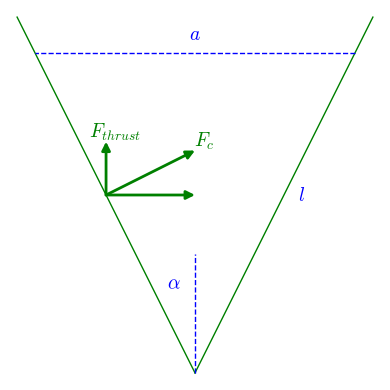
\includegraphics[width=0.48\textwidth]{Antipins_angle_en.png}
\caption{}{Antipin's angle}
\end{center}
\label{fig:Antipins_angle}
\end{wrapfigure}

    \section{Appendix D. The derivation of the thrust formula for the
honeycomb basing on the Antipin formula for the thrust of a metal
angle}\label{appendix-d.-the-derivation-of-the-thrust-formula-for-the-honeycomb-basing-on-the-antipin-formula-for-the-thrust-of-a-metal-angle}

    Antipin \cite{Antipin2012} gives an estimated calculation of the thrust
force of the ``corner'' using the Casimir formula, ``with the most
general and natural approximations known as PFA (Proximity Force
Approximation), or PAA (Pairwise Additive Approximation), calculation
method \cite{Intravaia2013}, \cite{Rodriguez2011}".

Casimir's interaction energy is given by
\[\delta\,E/L^2 = \hbar\,c\frac{\pi^2}{4\,a^3}\left\{\frac{-4}{24\times30}\right\}\]

Casimir's force
\[F_{c} = \hbar\,c\frac{-3\,\pi^2}{4\,a^4}\left\{\frac{-4}{24\times30}\right\}\]

Driving force of the metal corner

\[F_{thrust} = 2 \int F_{c} \, sin\, \alpha \,dS\]

\[dS = b\,dz\]

\[F_{thrust} = 2\, \frac{-3\,\pi^2\hbar c b}{4}\int\limits_{z_{min}}^{z_{max}} \left\{\frac{-4}{24\times30}\right\}\frac{sin\, \alpha}{\left(a\left(z\right)\right)^4}dz\]

Let's make a substitution

\[a\left(z\right) = 2\,z\,tg\, \alpha\]

\[F_{thrust} = 2\, \frac{-3\,\pi^2\hbar c b}{4}\int\limits_{z_{min}}^{z_{max}} \left\{\frac{-4}{24\times30}\right\}\frac{sin\, \alpha}{\left(2\,z\,tg \alpha\right)^4}dz\]

\[F_{thrust} = 2\, \frac{-3\,\pi^2\hbar c b}{4} \frac{sin\, \alpha}{\left(2\,tg\, \alpha\right)^4} \int\limits_{z_{min}}^{z_{max}} \left\{\frac{-4}{24\times30}\right\} \frac{dz}{z^4}\]

\[F_{thrust} = -2\cdot3\, \frac{\pi^2\hbar c b}{240} \frac{sin\, \alpha}{\left(2\,tg\, \alpha\right)^4} \left(\frac{1}{z^3}\right)\Bigg\rvert_{\,z_{min}}^{\,z_{max}} \]

    You can make a substitution \[z = l\, cos\, \alpha\]

\[F_{thrust} = -2\cdot3\, \frac{\pi^2\hbar c b}{240} \frac{sin\, \alpha}{2^4\left(tg\,\alpha\right)^4\left(cos\, \alpha\right)^3} \left(\frac{1}{l^3}\right)\Bigg\rvert_{\,l_{min}}^{\,l_{max}} \]

\[F_{thrust} = -2\cdot3\, \frac{\pi^2\hbar c b}{240} \frac{cos\, \alpha}{2^4\left(sin\, \alpha\right)^4} \left(\frac{1}{l^3}\right)\Bigg\rvert_{\,l_{min}}^{\,l_{max}} \]

\[F_{thrust} = \frac{\pi^2\hbar c b}{640} \frac{cos\, \alpha}{\left(sin\, \alpha\right)^4} \left(\frac{1}{l_{min}^3} - \frac{1}{l_{max}^3}\right)\]

Thus, the formula for the thrust of the corner is obtained basing on the
length of its wings.

Antipin indicates that the value of \(l_{min}\) is limited from below by
the "cutoff" level, which is determined technologically:

\begin{itemize}
\item
  by the accuracy of manufacturing of the plates (their roughness,
  degree of flatness), as well as
\item
  by the the minimum wavelength of photons that can effectively reflect
  the substance from which the corner is made (by \(k_m\) value).
\end{itemize}

    Investigating the dependence of the coefficient in the angle thrust
formula, which depends on the opening half angle \(\alpha\), it can be
seen that for a given length of the angle wings, it is more profitable
to make the minimum possible opening angle. However, for the purposes of
this work (study of the possibility of obtaining thrust using
nanocells), it is important to note that for a corner with a right angle
\(\alpha = {\pi}/{4}\), the coefficient
\(\left({cos\, \alpha}\right)\big/\left({\left(sin\, \alpha\right)^4}\right) = 2\sqrt{2}\).
Thus, composing a structure in the form of honeycombs from many
rectangular corners, it is shown that the thrust of the panel consisting
of rectangular honeycombs is not zero.

Indeed, a rectangular honeycomb with a cell size of \(b \times b\) and
with the same edge height equal to \(b = l_{max}\) can be imagined as a
combination of four corners with a half opening angle equal to
\(\alpha = {\pi}/{4}\). Driving force of the every corner

\[F_{thrust} = - \frac{\pi^2\hbar c l_{max}}{640} 2\sqrt{2} \left(\frac{1}{l_{min}^3} - \frac{1}{l_{max}^3}\right)\]

directed along the bisector of each angle must be multiplied by
\(sin\left({\pi}/{4}\right)={\sqrt{2}}\big/{2}\) and, when multiplied by
4, the thrust of one square "opened" cell will be equal to

\[F_{thrust} = - \frac{\pi^2\hbar c b}{640} 2\sqrt{2}\cdot4\,\frac{\sqrt{2}}{2} \left(\frac{1}{l_{min}^3} - \frac{1}{b^3}\right)\]

\[F_{thrust} = - \frac{\pi^2\hbar c b}{640} 2\cdot4\,\left(\frac{1}{l_{min}^3} - \frac{1}{b^3}\right)\]

\[F_{thrust} = - \frac{\pi^2\hbar c b}{80} \left(\frac{1}{l_{min}^3} - \frac{1}{b^3}\right)\]

So, the formula for the specific thrust of cells, obtained using the PFA
(Proximity Force Approximation) method, or PAA (Pairwise Additive
Approximation)

\[\frac{F_{thrust}}{S} = - \frac{\pi^2\hbar c}{80\, b} \left(\frac{1}{l_{min}^3} - \frac{1}{b^3}\right)\]

to some extent similar to the formula for the magnitude of the
two-dimensional Casimir effect on honeycombs, produced in the first part
of this work: at least the value of the exponent in the denominator is
the same.

\[\delta\,\frac{E}{V} \approx R\left(b \cdot k_m\right)\,\frac{\hbar\,c\,\pi}{b^4}\]

It should be noted here that this formula is obtained without taking
into account the finiteness of the cell edge height (in other words, in
the approximation of the infinite edge height), in contrast to the PFA
version of the formula for which the edge height is assumed to be equal
to the cell width.

The approximate correspondence of these formulas indicates that the
effect should also be observed at a finite height of the ribs, although
the dependence of the effect on this height may be the object of further
research.

Theoretically it is possible to achieve a greater value of thrust With a
panel of acute angled corners, but technologically the production of
panels from honeycombs seems to be simpler than the production of panels
from V-shaped corners.

    \begin{thebibliography}{99}

\bibitem{Casimir1948}
\textit{Casimir, H. B. G. (1948). On the attraction between two perfectly conducting plates. Proc. K. Ned. Akad. Wet. B 51, 793–5.
https://www.dwc.knaw.nl/DL/publications/PU00018547.pdf}

\bibitem{Boyer1968}
\textit{Boyer, T. H. (1968). Quantum electromagnetic zero-point energy of a conducting spherical shell and Casimir model for a charged particle. Phys. Rev. 174, 1764–76.}

\bibitem{Antipin2012}
\textit{Antipin A. V. (2012). RU 2 610 018 C2. Method for propulsion of bodies by Casimir effect and/or its analogue.}

\bibitem{Bikyalis1968}
\textit{A.Bikyalis (1968). Euler-Maclaurin summation formula for a function of many variables.  Lietuvos matematikos rinkinys. Литовский математический сборник. p.681
https://www.journals.vu.lt/LMJ/article/view/20600/19701}

\bibitem{Tuo2019}
\textit{Tuo Qu, Fang Liu, Yuechai Lin, Yidong Huang, "Metal nano-honeycomb fabricated by colloidal assembly and femtosecond-laser annealing," Proc. SPIE 10841, 9th International Symposium on Advanced Optical Manufacturing and Testing Technologies: Meta-Surface-Wave and Planar Optics, 108410A (30 January 2019); https://doi.org/10.1117/12.2508593}

\bibitem{Hrvoje2016}
\textit{Nikolic, Hrvoje (2016). "Proof that Casimir force does not originate from vacuum energy". Physics Letters B. 761: 197–202. arXiv:1605.04143. Bibcode:2016PhLB..761..197N. doi:10.1016/j.physletb.2016.08.036. S2CID 119265677.}

\bibitem{Intravaia2013}
\textit{F. Intravaia et al., Strong Casimir force reduction through metallic surface nanostructuring // Nature Comm, art. 2515, 4 (Sep. 2013) pp. 1-20}

\bibitem{Rodriguez2011}
\textit{A.W. Rodriguez, F. Capasso, S.G. Johnson, The Casimir effect in microstructured geometries // Nature Photonics, V.5, (Apr. 2011), p.211-221}

\end{thebibliography}


    % Add a bibliography block to the postdoc
    
    
    
\end{document}
